\documentclass[tikz,10pt,oneside,a4paper]{report}

% \usepackage[utf8]{inputenc} % specify input encoding, this should match the encoding of your editor
% \usepackage[]{fontenc}	    % specify the output encoding of PDF file.
\usepackage[english]{babel} % hyphenation patterns

% \usepackage{syntonly}
\usepackage{amsmath, amsthm, amssymb}
\usepackage{bm}	% bold math
\usepackage{enumitem}	% style of list item
\usepackage{fancyhdr}	% set header and footer
\usepackage{float}	% provide the placement option 'H', enforcing the placement exactly at that point of floating env.
%    \pagestyle{fancy}
\usepackage[colorlinks]{hyperref}   % make colored hyperlink
    \hypersetup{
	colorlinks = true,
	linkcolor = black,
	urlcolor = blue,
    }
\usepackage{listings}	% Code presentation
% \lstset{
%     language = TeX,
%     backgroundcolor = \color{white},
%     basicstyle = \footnotesize,
%     breakatwhitespace = false,	% automatics breaks at whitespace
%     breaklines = true,		% automatics line break
%     captionpos = b,		% caption-position at bottom
%     commentstyle = \color{blue},
%     escapeinside = {\%*}{*)},	% 
%     identifierstyle=,		% nothing happen
%     keepsapces = true,		% keep spaces in text
%     keywordstyle = \color{brown},
%     numbers = none,		% line numbers
%     numbersep = 5pt,		% how far line-numbers away from code
%     numberstyle = \tiny\color{gray}
%     stepnumebr = 2,		% If this option is 1, then each line will be numbered
%     stringstyle = \color{cyan},	% string literal style
%     tablesize = 2,		
% }
\usepackage{makeidx}
\usepackage{multicol}	% multicolumns environment
% \usepackage{tabbing}	% tabbing env.
\usepackage[dvipsnames]{xcolor}   % colored text
\usepackage{tikz}
    \usetikzlibrary{arrows,shapes,chains,positioning}
    \usetikzlibrary{decorations.markings}
% \usepackage{graphicx} % when used with tikz package, don't load
	% this one, otherwise it will be loaded twice, and causing errors.
\graphicspath{{figures/}}    % note the double {} here.
\usepackage{wrapfig}	% wrap figures with text

\usepackage{eso-pic}	% AddToShipoutPictureBG
\usepackage{geometry}	% set margin
    \geometry{left=2.5cm,right=2.5cm,top=2.5cm,bottom=2.5cm}  % margin
\usepackage{lipsum} % produce random text
% \lipsum[1-4]	% produce 4 paragraphs
\usepackage{tabularx}	% align cell of fixed width 
\usepackage[most]{tcolorbox}	% color box (background)
\tcbset{
%    frame code={},
%    center title,
    left=0pt,
    right=0pt,
    top=0pt,
    bottom=0pt,
    colback=gray!70,
    colframe=white,
%    width=\dimexpr\textwidth\relax,
%    enlarge left by=0mm,
%    boxsep=5pt,
%    arc=0pt, outer arc=0pt,
}

\newcommand{\TOC}{Table of Contents}
\newcommand{\rom}[1]{\expandafter\@slowromancap\romannumeral #1@}
\newcommand{\Rom}[1]{\uppercase\expandafter{\romannumeral #1\relax}}
\newcommand{\red}[1]{\textcolor{red}{#1}}
\newcommand{\green}[1]{\textcolor{green}{#1}}
\newcommand{\blue}[1]{\textcolor{blue}{#1}}
\newcommand{\package}[1]{\colorbox{gray!15!}{\textcolor{red}{\textbf{#1}}}}
\newcommand{\command}[1]{\colorbox{gray!15!}{\textcolor{OliveGreen}{\textbf{#1}}}}
\newcommand{\option}[1]{\colorbox{gray!15!}{\textcolor{RawSienna}{\textbf{#1}}}}
% add a 'Go to TOC' button in every page
\newcommand\AtPageUpperRight[1]{\AtPageUpperLeft{
    \put(\LenToUnit{\paperwidth},\LenToUnit{-0.1\paperheight}){#1}}}
\AddToShipoutPictureBG{
    \AtPageUpperRight{\put(-60,0){\hyperref[toc]{TOC}}}
}

\title{Hello World}
\author{Weibin Zhang \\ \url{weibin.zhang@stonybrook.edu} \\ 
\url{personal url} }
\date{\today}

% \setlength\parindent{0pt}

\begin{document}
\maketitle

\begin{multicols}{2}
    \tableofcontents\label{toc}    % to make a clickable toc, need hyperref package.
\end{multicols}


TODO:
\begin{itemize}
    \item style for code, for little chunks of code, for large chunks of code and their output.
\end{itemize}
\chapter{Introduction}
Introduce what \LaTeX is.

At the beginning of most documents there will be information about the
document itself, such as the title and date, and also information about the
authors, such as name, address, email etc. All of this type of information
within LaTeX is collectively referred to as \textit{top matter}. 

\section{Definition}
Following conventions will be used in this report:  \\
\package{package}   \\
\command|command|   \\
\option{option}	    \\

%%%%%%%%%%%%%%%%%%%%%%%%%%%%%%%%%%%%%%%%%%%%%%%%%%%%%%%%%%%%%%%%%%%%%%%%
\section{Packages}
While writing your document, you will probably find that there are some
areas where basic LaTeX cannot solve your problem. If you want to include
graphics, colored text or source code from a file into your document, you
need to enhance the capabilities of LaTeX. Such enhancements are called
packages. Some packages come with the LaTeX base distribution. Others are
provided separately. Modern TeX distributions come with a large number of
packages pre-installed. 

%%%%%%%%%%%%%%%%%%%%%%%%%%%%%%%%%%%%%%%%%%%%%%%%%%%%%%%%%%%%%%%%%%%%%%%%
\section{Box}
The key lies in \LaTeX{} is box, which is the smallest unit processed by
\LaTeX{}. Everything is thought as a box, and then aligned into page.

%%%%%%%%%%%%%%%%%%%%%%%%%%%%%%%%%%%%%%%%%%%%%%%%
\subsection{Introduction}
A \emph{box} is the \TeX term for an invisible container that can hold a
visible element, nothing, or other boxes. \emph{Glue} is the \TeX term for
an invisible connector that determines the separation between boxes. A 
visible element can be a letter, image, geometric shape, etc. \TeX builds 
pages by gluing boxes together. In a typical document, letter boxes are glues 
to other letter boxes to form words, which are then elastically glued to 
other words to form sentences. Sentences are broken into lines and placed 
in paragraph boxes. Elastic glue is squeezed or stretched to fully justify 
lines within paragraph boxes. Paragraph boxes are glued to diagram boxes, 
and so on.
\begin{figure}[htp]
    \centering
    \includegraphics[scale=0.7]{500px-Latex_boxed_characters}
\end{figure}

While it is true that boxes can hold other boxes, not all commands that can 
generate boxes be used within all other commands that can generate boxes. 
There are often workarounds for these limitations.

The size of a box is typically to the size and position of its contents,
but it doesn't have to be. Many box commands accept custom widths and/or
heights, and there are other commands that effect the shape and position 
of boxes. Boxes are placed relative to other boxes, while visible elements
are placed relative to the boxes which contains them.
\begin{figure}[htp]
    \centering
    \includegraphics[scale=0.5]{LaTeX_boxes_that_dont_match_their_contents}
\end{figure}
%%%%%%%%%%%%%%%%%%%%%%%%%%%%%%%%%%%%%%%%%%%%%%%%
\subsection{Boxes}

%%%%%%%%%%%%%%%%%%%%%%%%
\subsubsection{character boxes}
\TeX character boxes have three dimensional propreties:
\begin{itemize}
    \item \textbf{height} is the length between the baseline and the top of the box.
    \item \textbf{depth} is the length between the baseline and the bottom of the box.
    \item \textbf{width} is the width of the box.
\end{itemize}
\begin{figure}[htp]
    \centering
    \includegraphics[scale=0.7]{300px-charbox}
\end{figure}

%%%%%%%%%%%%%%%%%%%%%%%%
\subsubsection{parbox, minipage, and pbox}
A \command|\parbox| is a box of specific width formatted in paragraph mode. 
In paragraph mode, text is broken into lines and lines are broken into pages.
\command|\parbox[pos][height][contentpos]{width}{text}|

\option{width} defines the width of the paragraph box. Text will be broken 
into lines so that it fits within this width. 

\option{pos} selects which baseline to join. It can be \textbf{t}op, \textbf{b}ottom,
or \textbf{c}enter. 

\option{contentpos} positions the contents of the box within the box. It 
can be one of \textbf{c}enter, \textbf{t}op, \textbf{b}ottom or \textbf{s}pread. Note
that \option{contentpos} has no effect if the box is not larger than the
text it contains.


\command|\pbox[pos][height]{width}{text}|

\chapter{Basic}

%%%%%%%%%%%%%%%%%%%%%%%%%%%%%%%%%%%%%%%%%%%%%%%%%%%%%%%%%%%%%%%%%%%%%%%%
% Document classes
\section{Document classes}
\begin{description}[style=nextline]
    \item [article] 
	For articles in scientific journals, presentation, short
	reports, program documentation, invitations, etc
    \item [report]  
	For longer reports containing several chapters, small
	books, thesis, etc
    \item [book] 
	For real books
    \item [slides]
	For slides, this class uses big sans serif letters
    \item [letter]
	For letter
    \item [beamer]
	For presentations.
\end{description}
%%%%%%%%%%%%%%%%%%%%%%%%%%%%%%%%%%%%%%%%%%%%%%%%
\subsection{Document Class Options} 
\begin{description}[style=nextline]
    \item [11pt]
	Font size, default 10pt.
    \item [a4paper]
	Paper size, default letterpaper. Available options:
	a5paper, b5paper, executivepaper and legalpaper.
    \item [fleqn]
	Typesets displayed formula left-aligned instead of
	centered(default).
    \item [leqno]
	Places the numbering of formulas on the left hand side
	instead of the right(default).
    \item [titlepage, notitlepage]
	The article class does not start a new
	page by default, while report and book do.
    \item [twocolumn]
	Two columns, default one.
    \item [twoside,oneside]
	The article and report classes are single sides
	and the book class is double sided by default. 
    \item [landscape]
	landscape mode. default portrait.
    \item [openright,openany]
	Begin a chapter either only on right hand
	pages or on the next page available. This does not apply to
	\textit{article} class, as it doesn't know about chapters. The
	report class by default starts chapters on the next page available
	and the book class starts them on right hand pages.
    \item [draft,final]
	draft mode, which will speed up typesetting, because
	figures are not loaded, just indicated by a frame. In draft mode,
	\LaTeX{} indicates hyphenation and justification problems with a
	small square in the right-hand margin of the problem line so they
	can be located quickly.
\end{description}
%%%%%%%%%%%%%%%%%%%%%%%%%%%%%%%%%%%%%%%%%%%%%%%%
\subsection{Papersize}
\begin{description}
    \item [letterpaper]	$11 \times 8.5 $ in
    \item [legalpaper]	$14 \times 8.5 $ in
    \item [executivepaper]  $10.5 \times 7.25 $ in
    \item [a4paper] $20.7 \times 21$ in
    \item [a5paper] $21 \times 14.8$ in
    \item [b5paper] $25 \times 17.6$ in
\end{description}


%%%%%%%%%%%%%%%%%%%%%%%%%%%%%%%%%%%%%%%%%%%%%%%%%%%%%%%%%%%%%%%%%%%%%%%%
\section{Sections}
\LaTeX{} provides 7 levels of depth for defining sections.
\begin{description}[style=nextline]
    \item [part]
	level -1, not in letters.
    \item [chapter] 
	level 0, only books and reports.
    \item [section] 
	level 1, not in letters.
    \item [subsection] 
	level 2, not in letters.
    \item [subsubsection] 
	level 3, not in letters.
    \item [paragraph] 
	level 4, not in letters.
    \item [subparagraph] 
	level 5, not in letters.
\end{description}

%%%%%%%%%%%%%%%%%%%%%%%%%%%%%%%%%%%%%%%%%%%%%%%%
\subsection{Options}
    For some section with very long title, \LaTeX{} arrows you to give an
    optional extra version in the Table of Contents and any running heads.
    For example, \verb|\section[Short Name]{Very long title}|, with this
    command, \textbf{Short Name} will appears in \TOC{}, instead of the Very
    long title. 
% Special Characters 

Each sections command also has a "starred" version which does not produce
numbers. Because the *-form sectioning commands don't enter \TOC{}
automatically, \LaTeX{} offers two commands to insert such info directly
into a contents file: \\
\verb|\addtocontents{file}{text}| or
\verb|\addcontentsline{file}{type}{text}|
\begin{description}
    \item [file]    the extension of the contents file, usually toc, lof or
	lot.
    \item [type]    For \textit{lof} or \textit{lot},  \textit{figure} or
	\textit{table} is specified.
    \item [text]    Actually info written to \TOC{}.
\end{description}

%%%%%%%%%%%%%%%%%%%%%%%%%%%%%%%%%%%%%%%%%%%%%%%%
\subsection{\TOC{}}
One can modify the style of \TOC{}.

%%%%%%%%%%%%%%%%%%%%%%%%%%%%%%%%%%%%%%%%%%%%%%%%%%%%%%%%%%%%%%%%%%%%%%%%
\section{Special Characters and Phrases}
\begin{table}
    \centering
    \caption{Special Characters}
    \label{tab:spe_chars}
    \begin{tabular}{|cl|}
	\hline
	\textasciitilde	& \textbackslash{textasciitilde} or \textbackslash{\~{}\{\}}	\\
	\&  & \textbackslash{}\&    \\
	\#  & \textbackslash{}\#    \\
	\_  & \textbackslash{}\_    \\
	\$  & \textbackslash{}\$    \\
	\textbackslash{}    & \textbackslash{textbackslash} \\
	\%  & \textbackslash{}\%    \\
	\textasciicircum    & \textbackslash{textasciicircum} or \textbackslash{\^{}\{\}}  \\
	\{  & \textbackslash{}\{    \\
	\}  & \textbackslash{}\}    \\
	\hline
	\textless, \textgreater	& \textbackslash{textless}, \textbackslash{textgreater}	\\
	\hline
    \end{tabular}
\end{table}

\begin{description}[style=nextline]
    \item [\LaTeX{}]	\verb|\LaTeX{}| 
    \item [\~{}]	Non breakable space
    \item [\ldots]	\verb|\ldots|
\end{description}

%%%%%%%%%%%%%%%%%%%%%%%%%%%%%%%%%%%%%%%%%%%%%%%%
\subsection{Special Symbols}
\begin{table}
    \centering
    \begin{tabular}{ll}
	\verb|\oe, \OE|	&   \oe, \OE	\\
	\verb|\ae, \AE|	&   \ae, \AE	\\
	\verb|\aa, \AA|	&   \aa, \AA	\\
	\verb|\o, \O|	&   \o, \O	\\
	\verb|\l, \L|	&   \l, \L	\\
	\verb|\ss|	&   \ss	\\
	\verb|?`|	&   ?`	\\
	\verb|!`|	&   !`	\\
	\verb|\dag|	&   \dag	\\
	\verb|\ddag|	&   \ddag	\\
	\verb|\S|	&   \S	\\
	\verb|\P|	&   \P	\\
	\verb|\copyright|   &   \copyright	\\
	\verb|{\it \$}|	&   {\it \$}	\\
	\verb|{\it \&}|	&   {\it \&}	\\
	\verb|\i|	&   \i	\\
	\verb|\j|	&   \j	\\
    \end{tabular}
\end{table}

%%%%%%%%%%%%%%%%%%%%%%%%%%%%%%%%%%%%%%%%%%%%%%%%
\subsection{Space}
option to \verb|\\| like this \verb|\\[10pt]|	\\[10pt]
change the vertical distance between lines. \\
Horizontal space \verb|\hspace{1cm}|


Vertical space:	\\
This is \verb|\smallskip| 
\smallskip 
This is \verb|\medskip| 
\medskip
This is \verb|\bigskip|
\bigskip
End

%%%%%%%%%%%%%%%%%%%%%%%%%%%%%%%%%%%%%%%%%%%%%%%%
\subsection{Dashes}
\begin{description}
    \item[-]	hyphen 'double-quote'
    \item[-{}-]	dash denoting a range, e.g. 155--159
    \item[-{}-{}-]	punctuation dash---here it is.
\end{description}

%%%%%%%%%%%%%%%%%%%%%%%%%%%%%%%%%%%%%%%%%%%%%%%%
\subsection{Accents}
There are a variety of control sequences for producing accents.
\begin{table}
    \centering
    \begin{tabular}{ccc}
	{\bf accent}	& {\bf command}	& {\bf example}	\\
	acute	& \verb|\'{a}|	&   \'{a}   \\
	grave	& \verb|\`{a}|	&   \`{a}   \\
	umlaut	& \verb|\"{a}|	&   \"{a}   \\
		& \verb|\={a}|	&   \={a}  \\
		& \verb|\^{a}|	&   \^{a}   \\
		& \verb|\"{a}|	&   \"{a}   \\
		& \verb|\~{a}|	&   \~{a}   \\
		& \verb|\.{a}|	&   \.{a}   \\
		& \verb|\u{a}|	&   \u{a}   \\
		& \verb|\v{a}|	&   \v{a}   \\
		& \verb|\H{a}|	&   \H{a}   \\
		& \verb|\t{aa}|	&   \t{aa}   \\
		& \verb|\c{a}|	&   \c{a}   \\
		& \verb|\d{a}|	&   \d{a}   \\
		& \verb|\b{a}|	&   \b{a}   \\
    \end{tabular}
\end{table}
These accents {\bf cannot} be used within mathematical formulae, some
different control sequencys are used to produce accents within mathematics.

%%%%%%%%%%%%%%%%%%%%%%%%%%%%%%%%%%%%%%%%%%%%%%%%%%%%%%%%%%%%%%%%%%%%%%%%
\section{Alignment}
Command \verb|\begin{center} ... \end{center}| and \\
\verb|\begin{flushright} ... \end{flushright}| and \\
\verb|\begin{flushleft} ... \end{flushleft}| \\
to align in center, right and left

%%%%%%%%%%%%%%%%%%%%%%%%%%%%%%%%%%%%%%%%%%%%%%%%%%%%%%%%%%%%%%%%%%%%%%%%
\section{Font}
The default font used by Palin TeX is \textbf{cmr10}, Knuth only put 128 
glyphs in the fonts, and the char encoding is somewhat different from 
ASCII. So to play chars not in cmr10, you have to specify the texttype,
for example:
\verb|{\tt\string\TeX}|

%%%%%%%%%%%%%%%%%%%%%%%%%%%%%%%%%%%%%%%%%%%%%%%%
\subsection{{\it italic correction}}
\begin{lstlisting}[language=TeX]
{\it italicized\/} or {\sl slanting type\/} correction.
\end{lstlisting}
The control command \verb|\/| produces the so-called {\it italic correction}, 
which is recommended when changing font back from an {\it italic} or 
{\sl slanted} into a {\rm roman} or {\bf boldface} font, in order to produce
extra space to compensate for the way in which some {\it italic} and 
{\sl slanted} letters lean into the following blank space. However, this
italic correction should not be used before a comma or a full stop.

%%%%%%%%%%%%%%%%%%%%%%%%%%%%%%%%%%%%%%%%%%%%%%%%
\subsection{Families}
By default, \LaTeX{} use serif typeface(roman) font. Other font typefaces
(sans serif, typewriter, a.k.a monospace) can be used with some specific 
commands.
\textrm{serif(roman) family}	\\
\textsf{sans serif family}      \\
\texttt{typewriter(monospace) family}	\\
\ttfamily
switch to ttfamily  \\
\sffamily
switch to sffamily  \\
\rmfamily
switch back to default one. \\

To change the default fonts, use the commands:	\\
\verb|\renewcommand{\familydefault}{\sfdefault}|

%%%%%%%%%%%%%%%%%%%%%%%%%%%%%%%%%%%%%%%%%%%%%%%%
\subsection{Style}
\textmd{medium};    \\
\textbf{bold}; \\
\textup{upright};   \\
\textsl{slanted style, which makes the text look a bit like \textit{italics}
but not quite}; \\
\textsc{small caps}. \\
\underline{underline}	\\
The corresponding switch commands are:
\begin{lstlisting}[language=TeX]
\mdseries
\bfseries
\upshape 
\itshape or \it
\slshape or \sl
\scshape or \sc
\end{lstlisting}
If you look closely, you will notice that italic text is not only slanted
but that different letters are actually used (e.g. a and {\it a}). 
However, this is only true for serif text, not for sans-serif text. Text
that is only slanted without using different characters is called 
``slanted'' instead of ``italic''.

%%%%%%%%%%%%%%%%%%%%%%%%%%%%%%%%%%%%%%%%%%%%%%%%
\subsection{Size}
{\Huge Huge} \\
{\huge huge} \\
{\LARGE LARGE}	\\
{\Large Large}	\\
{\large large}	\\
{\small small}	\\
{\footnotesize footnotesize} \\
{\scriptsize scriptsize}	\\
{\tiny tiny} \\
{\normalsize normalsize (default)}    \\
All the sizes of other commands depends on the size of normal text.


%%%%%%%%%%%%%%%%%%%%%%%%%%%%%%%%%%%%%%%%%%%%%%%%%%%%%%%%%%%%%%%%%%%%%%%%
\section{Color}
To color text in \LaTeX{}, use \textcolor{red}{xcolor} package. There are 
two syntax to add color to text:
\begin{lstlisting}[language=TeX]
\colorbox{color}{text}	% background color
\textcolor{color}{text}	% text color
{\color{color} some text}
\textcolor{color!20!}{text}	% use 20% of choosed color
\end{lstlisting}
\red{red}, \green{green}, \blue{blue}.
\colorbox{blue!30}{blue}

\newpage
% \pagecolor{gray!50!}   % background
% \color{blue}	% text 
%%%%%%%%%%%%%%%%%%%%%%%%%%%%%%%%%%%%%%%%%%%%%%%%
\subsection{pagecolor}
Use command \verb|\pagecolor{colorg}| to set the background color of page.

{\color{red} For unknown reason, if I change the bg color with 
\verb|\pagecolor{color}|, the `Go to TOC' button will fail in the 
following pages (including the current one).}
% \lipsum[1-3]
\newpage
% \pagecolor{white} \color{black}

%%%%%%%%%%%%%%%%%%%%%%%%%%%%%%%%%%%%%%%%%%%%%%%%
\subsection{Basic colors names available in \LaTeX{}}
black, blue, brown, cyan, darkgray, gray, green, lightgray, lime, 
magenta, olive, orange, pink, purple, red, teal, violet, white, yellow.
% \box

%%%%%%%%%%%%%%%%%%%%%%%%%%%%%%%%%%%%%%%%%%%%%%%%%%%%%%%%%%%%%%%%%%%%%%%%
\section{Footer and Header}
Use command \verb|\pagestyle{style}| or \verb|\thispagestyle{style}| 
to set page style, the possible styles are:
\begin{description}[style=nextline]
    \item [plain]   default style. The header is empty and the footer
	contains page numbers in the center.
    \item [empty]   Both header and footer are cleared.  
    \item [headings]	Puts running headings on each page. The document
	style specifies what goes in the headings.
    \item [myheadings]	You specify what is to go in the heading with the
	\verb|\markboth| or the \verb|\markright| commands. 
	The footer is empty in this page style. The header
	contains the page number on right side (on even pages) or on left
	side (on odd pages) along with other user-supplied information;
	there is an exception for the first page of each chapter, where the
	footer contains centred page number while the header is blank.
\end{description}

\thispagestyle{fancy}   % set fancy style
\fancyhf{}  % reset current configuration
% the width of the horizonal line between head and contents.
\renewcommand{\headrulewidth}{2pt}
\renewcommand{\footrulewidth}{1pt}
% set header
\rhead{\leftmark}   
\lhead{\rightmark}  
\chead{\thepage}
\rfoot{\thepage}
\lfoot{left foot}
\cfoot{center foot}

For double-sided documents (books), use different command \verb|\fancyhead|
and \verb|fancyfoot| with several options.
\begin{lstlisting}[language=TeX]
\pagestyle{fancy}
\fancyhf{}
% show chapter name in the left of even pages and right of odd pages
\fancyhead[LE,RO] {\leftmark} 
% show section name in the right of even pages and left of odd pages
\fancyhead[RE,LO] {\rightmark} 
% show page number in foot center of even and odd pages
\fancyfoot[CE,CO] {\thepage}	
\end{lstlisting}

%\pagestyle{empty}


% set plain style attribute
% \fancypagestyle{plain} 

This is a footnote \footnote[1]{first footnote} \footnote[2]{second footnote}

The following commands can be used in the headers and footers:
\begin{description}[style=nextline]
    \item [\textbackslash{thepage}] Number of current page
    \item [\textbackslash{thechapter}] Number of current chapter
    \item [\textbackslash{thesection}] Number of current section
    \item [\textbackslash{chaptername}] chapter name
    \item [\textbackslash{leftmark}] Names and number of current top-level
	structure(e.g. \textit{Chapter for reports, Sectoin for articles})
	in uppercase letters.
    \item [\textbackslash{rightmark}] Names and number of current next to 
	top-level structure in uppercase letters.
\end{description}

%%%%%%%%%%%%%%%%%%%%%%%%%%%%%%%%%%%%%%%%%%%%%%%%
\subsection{Pagenumber}
\verb|\pagenumbering{...}|
\begin{description}
    \item [arabic]
    \item [roman]   lowercase
    \item [Roman]   Uppercase
    \item [alph]    lowercase English letters
    \item [Alph]    Uppercase
\end{description}

%%%%%%%%%%%%%%%%%%%%%%%%%%%%%%%%%%%%%%%%%%%%%%%%%%%%%%%%%%%%%%%%%%%%%%%%
\section{Length}

\subsection{Unit}
\begin{description}
    \item [\textbf{sp}] scaled point,  65535 sp = 1 pt
    \item [\textbf{pt}]	point, 1/72.27 in, or 0.0138 in or 0.3515 mm
    \item [\textbf{bp}] big point,  1 in = 72 bp
    \item [\textbf{dd}] didot point,  1157 dd = 1238 pt
    \item [\textbf{mm}] a millimeter
    \item [\textbf{pc}] pica,  1 pc = 12 pt = 4.218 mm
    \item [\textbf{cc}] cicero,  1 cc = 12 dd = 4.513 mm
    \item [\textbf{cm}] a centimeter
    \item [\textbf{in}] a inch = 25.4 mm
    \item [\textbf{ex}] roughtly the height of an `x' (lowercase) in the current \textbf{font}
    \item [\textbf{em}] roughtly the width of an `M' (Uppercase) in the current \textbf{font}
    \item [\textbf{mu}] math unit = 1/18 em, where \textbf{em} is taken from the math 
	symbols family.
\end{description}
Hou much a point is depends on whom you ask. \TeX{} thinks a point is the
72.27th part of an inch, which is 2.54 cm. On the other hand, PostScript
and Adobe think a point is the 72th part of an inch (which is a big point
in \TeX{}).

%%%%%%%%%%%%%%%%%%%%%%%%%%%%%%%%%%%%%%%%%%%%%%%%
\subsection{general length}
\begin{table}[htb]
    \centering 
    \begin{tabular}{cc}
	\verb|\hskip| {\it length}  & horitontal blank space of {\it length}	\\
	\verb|\vskip| {\it length}  & vertical blank space of {\it length}	\\
    \end{tabular}
\end{table}

Note: If the word following the horizontal skip happens to be \lq plus \rq then 
you will probably get an error message:
\begin{lstlisting}[language=TeX]
    ! Missing number, treated as zero.
\end{lstlisting}
To avoid it, typing `\verb|\hskip 20 mm \relax|'

%%%%%%%%%%%%%%%%%%%%%%%%%%%%%%%%%%%%%%%%%%%%%%%%
\subsection{Structured length}
\begin{description}
    \item [\textbackslash{}baselineskip]    Vertical distance between lines in a paragraph.
    \item [\textbackslash{}columnsep]	    column separation
    \item [\textbackslash{}columnwidth]	    the width of a column
    \item [\textbackslash{}evensidemargin]  
    \item [\textbackslash{}oddsidemargin]    
    \item [\textbackslash{}linewidth]    
    \item [\textbackslash{}lineskip]    
    \item [\textbackslash{}paperwidth]    
    \item [\textbackslash{}paperheight]    
    \item [\textbackslash{}parskip]	    Vertical space between paragraphs
    \item [\textbackslash{}tabcolsep]    
    \item [\textbackslash{}textheight]	    Height of the text area in the page
    \item [\textbackslash{}textwidth]    
    \item [\textbackslash{}topmargin]    
\end{description}
%%%%%%%%%%%%%%%%%%%%%%%%%%%%%%%%%%%%%%%%%%%%%%%%
\subsection{table}
Length between columns :
\verb|\setlength{\tabcolsep}|	

%%%%%%%%%%%%%%%%%%%%%%%%%%%%%%%%%%%%%%%%%%%%%%%%%%%%%%%%%%%%%%%%%%%%%%%%
\section{Space}
First note that, as a general rule, you should never put a blank space after
a left parenthesis or before a right parenthesis. If you were to put a blank
space in these places, then you run the risk that \TeX{} might start a new line
immediately after the left parenthesis or before the right parenthesis, 
leavin the parenthesis marooned at the beginning or end of a line.

\TeX{} has its own rules for deciding the lengths of blank spaces. For instance,
\TeX{} will put an extra amount of space after a full stop if it considers
that the full stop marks the end of a sentence.

The rule adopted by \TeX{} is to regard a period (full stop) as the end of a
sentence if it is preceded by a lowercase letter. If the period is preceded by
an uppercase letter then \TeX{} assumes that it is not a full stop but follows
the initials of somebody's name.

This works very well in most cases. However \TeX{} occasionally gets things
wrong. This happens with a number of common abbreviations (as in `Mr.~Smith' 
or in `etc.'), and, in particular, in the names of journals given in
abbreviated form (e.g., `Proc. Amer. Math. Soc.'). The way to overcome this
problem is to put a backslash before the blank space in question. Thus we
should type:
\begin{lstlisting}[language=TeX]
    Mr.\ Smith
    etc.\ and
    Proc.\ Amer.\ Math.\ Soc.
\end{lstlisting}

\TeX{} determines itself how to break up a paragraph into lines, and will
occasionally hyphenate long words where this is desirable. However it is
sometimes necessary to tell \TeX{} not to break at a particular blank space.
The special character used for this purpose is \textasciitilde. It represents 
a blank space at which \TeX is not allowed to break between lines. It is often 
desirable to use \textasciitilde in names where the forenames are represented 
by initials. Thus to obtain `W.~R.~Hamilton' it is best to type 
W.\textasciitilde R.\textasciitilde Hamilton.

%%%%%%%%%%%%%%%%%%%%%%%%%%%%%%%%%%%%%%%%%%%%%%%%%%%%%%%%%%%%%%%%%%%%%%%%
\section{Commands}

%%%%%%%%%%%%%%%%%%%%%%%%%%%%%%%%%%%%%%%%%%%%%%%%%%%%%%%%%%%%%%%%%%%%%%%%
\section{List}
Three are three kinds of list in \LaTeX{}: 

\subsubsection{itemize}
\begin{itemize}
    \item First item
    \item Another item
\end{itemize}

\subsubsection{enumerate}
\begin{enumerate}
    \item One
    \item Two
\end{enumerate}

\subsubsection{description}
\begin{description}
    \item[Foo] Foo 
    \item[Bar] Bar
    \item[description] \hfill \\
	Use \textbackslash{fill} so that the explanaion begins in newline.
\end{description}

%%%%%%%%%%%%%%%%%%%%%%%%%%%%%%%%%%%%%%%%%%%%%%%%
\subsection{Bullet}
One can change the bullet of a list easily without loading any package.

%%%%%%%%%%%%%%%%%%%%%%%%
\subsubsection{Unordered lists}
\begin{itemize}
    \item[--] dash
    \item[$\ast$] asterisk
    \item[$\alpha$] Any math character
    \item[a] Char
\end{itemize}

%%%%%%%%%%%%%%%%%%%%%%%%
\subsubsection{Ordered lists}

roman:	\\
\begin{enumerate}[label = (\roman*)]	% this option require enumitem package
    \item enumerate
    \item Option (A1) specify label 'A'.
\end{enumerate}

Roman:
\begin{enumerate}[label=(\Roman*)]
    \item One
    \item Two
\end{enumerate}

arabic:
\begin{enumerate}[label = (\arabic*)]
    \item One
    \item Two
\end{enumerate}

alph:
\begin{enumerate}[label = (\alph*)]
    \item a
    \item b
\end{enumerate}

Alph:
\begin{enumerate}[label = (\Alph*)]
    \item a
    \item b
\end{enumerate}

%%%%%%%%%%%%%%%%%%%%%%%%%%%%%%%%%%%%%%%%%%%%%%%%%%%%%%%%%%%%%%%%%%%%%%%%
\section{Table}

{\color{red}??? How to wrap text within a table cell ???}

\verb|\toprule, \midrule, \bottomrule| used as seperation line.

%%%%%%%%%%%%%%%%%%%%%%%%%%%%%%%%%%%%%%%%%%%%%%%%
\subsection{tabbing}
\emph{tabbing} env. can also produce table format:
\begin{tabbing}
    \textbf{AbiWord}\quad\= : \= A word processor\kill \\
    \textbf{\TeX}\quad	 \> : \> A typesetting program \\[5pt]
    \textbf{Emacs}\quad	 \> : \> A text editor \\[5pt]
			 \>   \> \quad\= a programming env. \\[5pt]
			 \>   \>      \> a mail reader \\[5pt]
			 \>   \>      \> and a lot more besides \\[5pt]
    \textbf{AbiWord}\quad\> : \> A word processor
\end{tabbing}

The alighment of text can be: l,c,r or p{length}

\begin{center}
    \begin{tabular}{lp{6cm}}
	Planet	& Features\tabularnewline[8pt]
	Mercury	& \raggedright	Lunar like crust \\
				Crustal faulting \\
				Small magnetic fiels\tabularnewline[3pt]
		& Guess what's this \\
    \end{tabular}
\end{center}

%%%%%%%%%%%%%%%%%%%%%%%%%%%%%%%%%%%%%%%%%%%%%%%%
\subsection{Multi-columns or rows}
\verb|multicolumn{num}{pos}{item}|
\begin{center}
    \begin{tabular}{|l|r|r|}
	\hline
	Planet	& \multicolumn{2}{c|}{Distance from sum (km)}\\
	\cline{2-3} 
		& Maximum   & Minimum   \\
	\hline
	Mercury	& 69400000  & 46800000	\\
	Pluto	& 734600000 & 4461000000    \\
	\hline
    \end{tabular}
\end{center}
Similarly, we can apply \verb|multirow[pos]{num}{*}{item}| when include
\emph{multirow} package.

\begin{center}
    \begin{tabular}{|l|r|r|}
	\hline
		& \multicolumn{2}{p{3.5cm}|}{\centering Distance from sum
	        \\ (kilometer)}\\
	\cline{2-3} 
	\multicolumn{1}{|c|}{Planet}	& \multicolumn{1}{c|}{Maximum}	
		& \multicolumn{1}{c|}{Minimum}   \\
	\hline
	Mercury	& 69400000  & 46800000	\\
	Pluto	& 734600000 & 4461000000    \\
	\hline
    \end{tabular}
\end{center}

\begin{center}
    \begin{tabular}{|c|r@{--}l|}
	\hline
	Height	& \multicolumn{2}{c|}{Ideal weight} \\
	(cm)	& \multicolumn{2}{c|}{(kg)} \\
	\hline
	155 & 53.5  & 64    \\
	160 & 56    & 67    \\
	190 & 78    & 92.5  \\
	\hline
    \end{tabular}
\end{center}

%%%%%%%%%%%%%%%%%%%%%%%%%%%%%%%%%%%%%%%%%%%%%%%%
\subsection{alignment}
Using package \textbf{tabularx}, one can manipulate the alignment of the
cells.

flush left fixed width:
\verb|\newcolumntype{L}[1]{>{\raggedright\arraybackslash}p{#1}}|

center fixed width:
\verb|\newcolumntype{C}[1]{>{\centering\arraybackslash}p{#1}}|

flush right fixed width:
\verb|\newcolumntype{R}[1]{>{\raggedleft\arraybackslash}p{#1}}|

\newcolumntype{L}[1]{>{\raggedright\arraybackslash}p{#1}}
\newcolumntype{C}[1]{>{\centering\arraybackslash}p{#1}}
\newcolumntype{R}[1]{>{\raggedleft\arraybackslash}p{#1}}

\begin{tabular}{|L{1cm}|C{2cm}|R{3cm}|}
    \hline
    1cm width	& 2cm width & 3cm width	\\
    \hline
    left    & center	& right	\\
    \hline
\end{tabular}

%%%%%%%%%%%%%%%%%%%%%%%%%%%%%%%%%%%%%%%%%%%%%%%%
\subsection{centering a wide table}
To center a very wide table, you can take the following ways:
\begin{itemize}
    \item \verb|\makebox[\textwidth][c]{<table>}|
    \item use adjustbox (from package \emph{adjustbox})
	\begin{verbatim}
	\begin{adjustbox}{center}
	    \begin{tabular}{ccc}
		table content
	    \end{tabular}
	\end{adjustbox}
	\end{verbatim}
    \item \verb|\centerline{<table>}|
\end{itemize}
%%%%%%%%%%%%%%%%%%%%%%%%%%%%%%%%%%%%%%%%%%%%%%%%%%%%%%%%%%%%%%%%%%%%%%%%
\section{Figure}

%%%%%%%%%%%%%%%%%%%%%%%%%%%%%%%%%%%%%%%%%%%%%%%%
\subsection{wrapfig}
Surrounding figures with text using package \emph{wrapfig}. Note
that text can't follow the wrapfig env. directly.

\begin{wrapfigure}{L}{0.3\textwidth}
    \centering 
    \includegraphics[width=0.25\textwidth]{frog}
    \caption{\label{fig:frog}A frog}
\end{wrapfigure}
% note the blank line here. text can't follow the wrapfig environment directly.

\lipsum[1]

\begin{wrapfigure}{R}{0.3\textwidth}
    \centering 
    \includegraphics[width=0.25\textwidth]{frog}
    \caption{\label{fig:frog}A frog}
\end{wrapfigure}

\lipsum[2]


%%%%%%%%%%%%%%%%%%%%%%%%%%%%%%%%%%%%%%%%%%%%%%%%%%%%%%%%%%%%%%%%%%%%%%%%
\section{Equation}

%%%%%%%%%%%%%%%%%%%%%%%%%%%%%%%%%%%%%%%%%%%%%%%%%%%%%%%%%%%%%%%%%%%%%%%%
\section{Code}

%%%%%%%%%%%%%%%%%%%%%%%%%%%%%%%%%%%%%%%%%%%%%%%%
\subsection{Verbatim}
The default tool to display code in \LaTeX{} is \textbf{verbatim}, which
generates an output in monospaced font. 
\begin{verbatim}
Tex enclodes inside \texttt{verbatim} envi. is printed directl and all
\LaTeX{} commands are ignored.
\end{verbatim}

A starred version of verbatim envi. will produce slightly different output
where white spaces are emphasized with a special symbol.
\begin{verbatim*}
Tex enclodes inside \texttt{verbatim} envi. is printed directl and all
\LaTeX{} commands are ignored.
\end{verbatim*}

Verbatim-like text can also be used in paragraph by means of the
\verb|\verb| command. Any charactre, except letters and *, can be used as
delimiter. For instance \verb+Delimiter+ use + as delimiter.

%%%%%%%%%%%%%%%%%%%%%%%%%%%%%%%%%%%%%%%%%%%%%%%%
\subsection{Highlighting code: listings package}
To produce highlight code, we need \textbf{listings}
\begin{lstlisting}[language=Python]
    import numpy as np

    def f(x1, x2):
	if x1 > x2:
	    print "Hello World"

    a=4, b=5
    f(b, a)
\end{lstlisting}

%%%%%%%%%%%%%%%%%%%%%%%%%%%%%%%%%%%%%%%%%%%%%%%%
\subsection{Importing code from a file}
To import code from files, using command \verb|\lstinputlisting|.
\begin{lstlisting}[language=TeX]
\lstinputlisting[language=Python]{hello_wrold.py}
\lstinputlisting[language=Python, caption = Python]{hello_wrold.py}
\lstinputlisting[language=Python, firstline=2, lastline=12]{hello_wrold.py}
\end{lstlisting}

%%%%%%%%%%%%%%%%%%%%%%%%%%%%%%%%%%%%%%%%%%%%%%%%
\subsection{Code Style}
\textbf{listings} is highly customisable.  
\begin{lstlisting}[language=TeX]
\definecolor{codegreen}{rgb}{0,0.6,0}
\definecolor{codegray}{rgb}{0.5,0.5,0.5}
\definecolor{codepurple}{rgb}{0.58,0,0.82}
\definecolor{backcolour}{rgb}{0.95,0.95,0.92}

\lstdefinestyle{mystyle}{
    backgroundcolor=\color{backcolour},   
    commentstyle=\color{codegreen},
    keywordstyle=\color{magenta},
    numberstyle=\tiny\color{codegray},
    stringstyle=\color{codepurple},
    basicstyle=\footnotesize,
    breakatwhitespace=false,         
    breaklines=true,                 
    captionpos=b,                    
    keepspaces=true,                 
    numbers=left,                    
    numbersep=5pt,                  
    showspaces=false,                
    showstringspaces=false,
    showtabs=false,                  
    tabsize=2
}

\lstset{style=mystyle}
\end{lstlisting}

%%%%%%%%%%%%%%%%%%%%%%%%%%%%%%%%%%%%%%%%%%%%%%%%%%%%%%%%%%%%%%%%%%%%%%%%
\section{Box}
Use \verb|\makebox| to fit wide table or figures.

\makebox[\textwidth]{
    \begin{tabular}{cc}
	a very long sentences that will fill up the cell, but it will still be centerized.  & this it the right cell that will exceed the right margin.
    \end{tabular}
}
%%%%%%%%%%%%%%%%%%%%%%%%%%%%%%%%%%%%%%%%%%%%%%%%%%%%%%%%%%%%%%%%%%%%%%%%
\section{Miscellaneous}
\verb|\rule{length}{width}|

{\color{red}	\rule{\linewidth}{0.5mm} }
%%%%%%%%%%%%%%%%%%%%%%%%%%%%%%%%%%%%%%%%%%%%%%%%%%%%%%%%%%%%%%%%%%%%%%%%
\section{Reference}
reference command :
\verb|\cite, \ref, \pageref and \label|
Put \verb|\label| in argument of \verb|\section| for cross-referencing:
\verb|\section{\label{}}|

%%%%%%%%%%%%%%%%%%%%%%%%%%%%%%%%%%%%%%%%%%%%%%%%%%%%%%%%%%%%%%%%%%%%%%%%
\section{Bibliography}
to cite a bibliography, use the \verb|\cite| command. 
Please refer to \cite{wiki} or \cite[option]{wiki}.

%%%%%%%%%%%%%%%%%%%%%%%%%%%%%%%%%%%%%%%%%%%%%%%%
\subsection{BIBTeX}
Another way to cite bibliography is using BIBTeX. \\
BIBTeX style:
\begin{description}
    \item [plain] Entries sorted alphabetically with numeric labels.
    \item [unsrt] Entries printed in order of citation.
    \item [alpha] Use author's name and the year of publication as labels.
    \item [abbrv] compact style, first name, month, and journal names are
	abbrevitated
    \item [acm]	it hse author name in small caps, and numbers as labels.
    \item [apalike] require \emph{apalike} package. Entries formatted
	alphabetically, last name first, each entry having a hanging
	indentation and no label.
\end{description}

To run BIBTeX with \LaTeX{}, (\Rom{1})\  one needs to run \LaTeX{} firstly to
generate a list of \textbackslash{}cite references in its auxiliary file
.aux. (\Rom{2})\  Then run BIBTeX to read the auxiliary file, looking up the references
in the database, and write results into .bbl file (formatted according to
the format specified in the .bst style file). (\Rom{3})\  Run \LaTeX{} again to read the
.bbl reference file. (\Rom{4})\  Finally run \LaTeX{} a third time, resolving all
reference. 

\begin{thebibliography}{9}
\bibitem{wiki}
    wikipedia.com.
\end{thebibliography}

\chapter{Math}

%%%%%%%%%%%%%%%%%%%%%%%%%%%%%%%%%%%%%%%%%%%%%%%%%%%%%%%%%%%%%%%%%%%%%%%%
\section{Font}
Fonts in mathematical mode.
\begin{description}
    \item [\textbackslash{}mathit]  italic (default)
    \item [\textbackslash{}mathrm]  roman
	\[
	    \mathrm ABCDEFGHIJKLMNOPQRSTUVWXYZ
	    \]
	\verb|\rm|
	\[
	    \rm ABCDEFGHIJKLMNOPQRSTUVWXYZ
	    \]
    \item [\textbackslash{}mathbf]  bold
    \item [\textbackslash{}mathsf]  sans serif
	\[
	    \mathsf ABCDEFGHIJKLMNOPQRSTUVWXYZ
	    \]
	\verb|\sf|
	\[
	    \sf ABCDEFGHIJKLMNOPQRSTUVWXYZ
	    \]
    \item [\textbackslash{}mathtt]  typewritter
    \item [\textbackslash{}mathcal] calligraphic (upper case only)
	\[
	    \mathcal ABCDEFGHIJKLMNOPQRSTUVWXYZ
	    \]
	\verb|\cal|
	\[
	    \cal ABCDEFGHIJKLMNOPQRSTUVWXYZ
	    \]
\end{description}
The recommended way to obtain ordinary text in displayed mathematical 
formulae is to use \verb|\hbox|.
\[
    M^\bot = \{ f \in V' : f(m) = 0 \hbox{ for all } m \in M \}.
    \]
Note the space before and after 'for all' in the input.

\subsection{Space}
\begin{lstlisting}[language=TeX]
    \begin{equation*}
	\begin{aligned}
	    f(x) =& x^2\! + 3x\! + 2 \\
	    f(x) =& x^2 + 3x + 2 \\
	    f(x) =& x^2\, + 3x\, + 2 \\
	    f(x) =& x^2\: + 3x\: + 2 \\
	    f(x) =& x^2\; + 3x\; + 2 \\
	    f(x) =& x^2\ + 3x\ + 2 \\
	    f(x) =& x^2\quad + 3x\quad + 2 \\
	    f(x) =& x^2\qquad + 3x\qquad + 2 \\
	\end{aligned}
    \end{equation}
\end{lstlisting}

\begin{equation*}
    \begin{aligned}
	f(x) =& x^2\! + 3x\! + 2 \\
	f(x) =& x^2 + 3x + 2 \\
	f(x) =& x^2\, + 3x\, + 2 \\
	f(x) =& x^2\: + 3x\: + 2 \\
	f(x) =& x^2\; + 3x\; + 2 \\
	f(x) =& x^2\ + 3x\ + 2 \\
	f(x) =& x^2\quad + 3x\quad + 2 \\
	f(x) =& x^2\qquad + 3x\qquad + 2 \\
    \end{aligned}
\end{equation*}

%%%%%%%%%%%%%%%%%%%%%%%%%%%%%%%%%%%%%%%%%%%%%%%%%%%%%%%%%%%%%%%%%%%%%%%%
\section{Symbols}

%%%%%%%%%%%%%%%%%%%%%%%%%%%%%%%%%%%%%%%%%%%%%%%%
\subsection{Greek Letters}
\begin{table}[!htbp]
    \centering
    \begin{tabular}{lp{2cm}lp{2cm}}
	\verb|\epsilon|	& $\epsilon$	& \verb|\varepsilon|	& $\varepsilon$    \\
	\verb|\theta|	& $\theta$	& \verb|\vartheta|	& $\vartheta$   \\
	\verb|\pi|	& $\pi$		& \verb|\varpi|		& $\varpi$    \\
	\verb|\rho|	& $\rho$	& \verb|\varrho|	& $\varrho$    \\
	\verb|\sigma|	& $\sigma$	& \verb|\varsigma|	& $\varsigma$    \\
	\verb|\phi|	& $\phi$	& \verb|\varphi|	& $\varphi$    \\
	\hline
	\verb|\zeta|	& $\zeta$	& \verb|\iota|		& $\iota$    \\
	\verb|\kappa|	& $\kappa$	& \verb|\xi|		& $\xi$    \\
	\verb|o|	& $o$		& \verb|\upsilon|	& $\upsilon$    \\
	\verb|\chi|	& $\chi$	& \verb|\psi|		& $\psi$    \\
    \end{tabular}
\end{table}

\subsection{Uppercase Greek Letters}
\begin{table}[H]
    \centering 
    \begin{tabular}{lp{2cm}lp{2cm}lp{2cm}}
	\verb|\Gamma|	& $\Gamma$  &
	\verb|\Xi|	& $\Xi$  &
	\verb|\Phi|	& $\Phi$    \\
	\verb|\Delta|	& $\Delta$  &
	\verb|\Pi|	& $\Pi$  &
	\verb|\Psi|	& $\Psi$    \\
	\verb|\Theta|	& $\Theta$  &
	\verb|\Sigma|	& $\Sigma$  &
	\verb|\Omega|	& $\Omega$	\\
	\verb|\Lambda|	& $\Lambda$  &
	\verb|\Upsilon|	& $\Upsilon$  &
	&   \\
    \end{tabular}
\end{table}

\subsection{Miscellaneous Symbols}
\begin{table}[!htbp]
    \centering
    \begin{tabular}{lp{2cm}lp{2cm}lp{2cm}}
	\verb|\aleph|	& $\aleph$	&
	\verb|\prime|	& $\prime$	&
	\verb|\forall|	& $\forall$	    \\
	\verb|\hbar|	& $\hbar$	& 
	\verb|\emptyset|	& $\emptyset$	& 
	\verb|\exists|	& $\exists$	    \\ 
	\verb|\imath|	& $\imath$	& 
	\verb|\nabla|	& $\nabla$	&   
	\verb|\neg|	& $\neg$	    \\ 
	\verb|\jmath|	& $\jmath$	& 
	\verb|\surd|	& $\surd$	& 
	\verb|\flat|	& $\flat$	    \\ 
	\verb|\ell|	& $\ell$	& 
	\verb|\top|	& $\top$	& 
	\verb|\natural|	& $\natural$	    \\ 
	\verb|\wp|	& $\wp$	& 
	\verb|\bot|	& $\bot$	& 
	\verb|\sharp|	& $\sharp$	    \\ 
	\verb|\Re|	& $\Re$	& 
	\verb/\|/	& $\|$	& 
	\verb|\clubsuit|	& $\clubsuit$	    \\
	\verb|\Im|	& $\Im$	& 
	\verb|\angle|	& $\angle$	& 
	\verb|\diamondsuit|	& $\diamondsuit$    \\
	\verb|\partial|	& $\partial$	& 
	\verb|\triangle|	& $\triangle$	& 
	\verb|\heartsuit|	& $\heartsuit$	\\
	\verb|\infty|	& $\infty$	& 
	\verb|\backslash|	& $\backslash$	& 
	\verb|\spadesuit|	& $\spadesuit$	\\
    \end{tabular}
\end{table}
	
%%%%%%%%%%%%%%%%%%%%%%%%%%%%%%%%%%%%%%%%%%%%%%%%
\subsection{``Large" Operators}
\begin{table}[!htbp]
    \centering
    \begin{tabular}{lp{2cm}lp{2cm}lp{2cm}}
	\verb|\sum|	    & $\sum$	&
	\verb|\bigcap|	    & $\bigcap$	&
	\verb|\bigodot|	    & $\bigodot$	\\
	\verb|\prod|	    & $\prod$	&
	\verb|\bigcup|	    & $\bigcup$	&
	\verb|\bigotimes|   & $\bigotimes$	\\
	\verb|\coprod|	    & $\coprod$	&
	\verb|\bigsqcup|    & $\bigsqcup$	&
	\verb|\bigoplus|    & $\bigoplus$	\\
	\verb|\int|	    & $\int$	&
	\verb|\bigvee|	    & $\bigvee$	&
	\verb|\biguplus|    & $\biguplus$	\\
	\verb|\oint|	    & $\oint$	&
	\verb|\bigwedge|    & $\bigwedge$	&
	&   \\
    \end{tabular}
\end{table}


%%%%%%%%%%%%%%%%%%%%%%%%%%%%%%%%%%%%%%%%%%%%%%%%
\subsection{Binary Operators}
\begin{table}[H]
    \centering
    \begin{tabular}{lp{2cm}lp{2cm}lp{2cm}}
	\verb|\pm|	    & $\pm$	&
	\verb|\cap|	    & $\cap$	&
	\verb|\vee|	    & $\vee$	\\
	\verb|\mp|	    & $\mp$	&
	\verb|\cup|	    & $\cup$	&
	\verb|\wedge|	    & $\wedge$	\\
	\verb|\setminus|    & $\setminus$	&
	\verb|\uplus|	    & $\uplus$	&
	\verb|\oplus|	    & $\oplus$	\\
	\verb|\cdot|	    & $\cdot$	&
	\verb|\sqcap|	    & $\sqcap$	&
	\verb|\ominus|	    & $\ominus$	\\
	\verb|\times|	    & $\times$	&
	\verb|\sqcup|	    & $\sqcup$	&
	\verb|\ominus|	    & $\ominus$	\\
	\verb|\ast|	    & $\ast$	&
	\verb|\triangleleft|	    & $\triangleleft$	&
	\verb|\oslash|	    & $\oslash$	\\
	\verb|\star|	    & $\star$	&
	\verb|\triangleright|	    & $\triangleright$	&
	\verb|\odot|	    & $\odot$	\\
	\verb|\diamond|	    & $\diamond$	&
	\verb|\wr|	    & $\wr$	&
	\verb|\dagger|	    & $\dagger$	\\
	\verb|\circ|	    & $\circ$	&
	\verb|\bigcirc|	    & $\bigcirc$	&
	\verb|\ddagger|	    & $\ddagger$	\\
	\verb|\bullet|	    & $\bullet$	&
	\verb|\bigtriangleup|	    & $\bigtriangleup$	&
	\verb|\amalg|	    & $\amalg$	\\
	\verb|\div|	    & $\div$	&
	\verb|\bigtriangledown|	    & $\bigtriangledown$	&
	&   \\
    \end{tabular}
\end{table}
%%%%%%%%%%%%%%%%%%%%%%%%%%%%%%%%%%%%%%%%%%%%%%%%
\subsection{Standard Functions and Embedded Text}
\begin{table}[!htbp]
    \centering
    \begin{tabular}{lp{2cm}lp{2cm}lp{2cm}}
	\verb|\arccos|	& $\arccos$ &
	\verb|\arcsin|	& $\arcsin$ & 
	\verb|\arctan|	& $\arctan$	\\ 
	\verb|\arg|	& $\arg$    & 
	\verb|\cos|	& $\cos$    & 
	\verb|\cosh|	& $\cosh$	\\ 
	\verb|\cot|	& $\cot$    & 
	\verb|\csc|	& $\csc$    & 
	\verb|\deg|	& $\deg$	\\ 
	\verb|\det|	& $\det$    & 
	\verb|\exp|	& $\exp$    & 
	\verb|\gcd|	& $\gcd$	\\ 
	\verb|\hom|	& $\hom$    & 
	\verb|\inf|	& $\inf$    & 
	\verb|\ker|	& $\ker$	\\ 
	\verb|\lg|	& $\lg$	& 
	\verb|\lim|	& $\lim$    & 
	\verb|\liminf|	& $\liminf$	\\ 
	\verb|\limsup|  & $\limsup$ & 
	\verb|\ln|	& $\ln$	&   
	\verb|\log|	& $\log$	\\ 
	\verb|\max|	& $\max$    & 
	\verb|\min|	& $\min$    & 
	\verb|\Pr|	& $\Pr$		\\   
	\verb|\sec|	& $\sec$    & 
	\verb|\sin|	& $\sin$    & 
	\verb|\sinh|	& $\sinh$	\\ 
	\verb|\sup|	& $\sup$    & 
	\verb|\tan|	& $\tan$    & 
	\verb|\tanh|	& $\tanh$	\\
    \end{tabular}
\end{table}

%%%%%%%%%%%%%%%%%%%%%%%%%%%%%%%%%%%%%%%%%%%%%%%%
\subsection{Relations}
\begin{table}[!htbp]
    \centering
    \begin{tabular}{lp{2cm}lp{2cm}lp{2cm}}
	\verb|\leq|	& $\leq$ &
	\verb|\geq|	& $\geq$ & 
	\verb|\equiv|	& $\equiv$	\\ 
	\verb|\prec|	& $\prec$    & 
	\verb|\succ|	& $\succ$    & 
	\verb|\sim|	& $\sim$	\\ 
	\verb|\preceq|	& $\preceq$    & 
	\verb|\succeq|	& $\succeq$    & 
	\verb|\simeq|	& $\simeq$	\\ 
	\verb|\ll|	& $\ll$    & 
	\verb|\gg|	& $\gg$    & 
	\verb|\asymp|	& $\asymp$	\\ 
	\verb|\subset|	& $\subset$    & 
	\verb|\supset|	& $\supset$    & 
	\verb|\approx|	& $\approx$	\\ 
	\verb|\subseteq|	& $\subseteq$	& 
	\verb|\supseteq|	& $\supseteq$    & 
	\verb|\cong|	& $\cong$	\\ 
	\verb|\sqsubseteq|  & $\sqsubseteq$ & 
	\verb|\sqsupseteq|	& $\sqsupseteq$	&   
	\verb|\bowtie|	& $\bowtie$	\\ 
	\verb|\in|	& $\in$    & 
	\verb|\ni|	& $\ni$    & 
	\verb|\propto|	& $\propto$		\\   
	\verb|\vdash|	& $\vdash$    & 
	\verb|\dashv|	& $\dashv$    & 
	\verb|\models|	& $\models$	\\ 
	\verb|\smile|	& $\smile$    & 
	\verb|\mid|	& $\mid$    & 
	\verb|\doteq|	& $\doteq$	\\
	\verb|\frown|	& $\frown$    & 
	\verb|\parallel|	& $\parallel$    & 
	\verb|\perp|	& $\perp$	\\
    \end{tabular}
\end{table}

%%%%%%%%%%%%%%%%%%%%%%%%%%%%%%%%%%%%%%%%%%%%%%%%
\subsection{Negated Relations}
\begin{table}[!htbp]
    \centering
    \begin{tabular}{lp{2cm}lp{2cm}lp{2cm}}
	\verb|\not<|		& $\not<$ &
	\verb|\not>|		& $\not>$ & 
	\verb|\not=|		& $\not=$	\\ 
	\verb|\not\leq|		& $\not\leq$ &
	\verb|\not\geq|		& $\not\geq$ & 
	\verb|\not\equiv|	& $\not\equiv$	\\ 
	\verb|\not\prec|	& $\not\prec$    & 
	\verb|\not\succ|	& $\not\succ$    & 
	\verb|\not\sim|		& $\not\sim$	\\ 
	\verb|\not\preceq|	& $\not\preceq$    & 
	\verb|\not\succeq|	& $\not\succeq$    & 
	\verb|\not\simeq|	& $\not\simeq$	\\ 
	\verb|\not\subset|	& $\not\subset$    & 
	\verb|\not\supset|	& $\not\supset$    & 
	\verb|\not\approx|	& $\not\approx$	\\ 
	\verb|\not\subseteq|    & $\not\subseteq$	& 
	\verb|\not\supseteq|    & $\not\supseteq$    & 
	\verb|\not\cong|	& $\not\cong$	\\ 
	\verb|\not\sqsubseteq|  & $\not\sqsubseteq$ & 
	\verb|\not\sqsupseteq|  & $\not\sqsupseteq$	&   
	\verb|\not\asymp|	& $\not\asymp$	\\ 
    \end{tabular}
\end{table}

%%%%%%%%%%%%%%%%%%%%%%%%%%%%%%%%%%%%%%%%%%%%%%%%
\subsection{Arrows}
\begin{table}[H]
    \centering
    \begin{tabular}{lp{2cm}lp{2cm}lp{2cm}}
	\verb|\leftarrow|	& $\leftarrow$	&
	\verb|\longleftarrow|	& $\longleftarrow$	&
	\verb|\uparrow|		& $\uparrow$	    \\
	\verb|\Leftarrow|	& $\Leftarrow$	&
	\verb|\Longleftarrow|	& $\Longleftarrow$	&
	\verb|\Uparrow|		& $\Uparrow$	    \\
	\verb|\rightarrow|	& $\rightarrow$	&
	\verb|\longrightarrow|	& $\longrightarrow$	&
	\verb|\downarrow|	& $\downarrow$	    \\
	\verb|\Rightarrow|	& $\Rightarrow$	&
	\verb|\Longrightarrow|	& $\Longrightarrow$	&
	\verb|\Downarrow|	& $\Downarrow$	    \\
	\verb|\leftrightarrow|	& $\leftrightarrow$	&
	\verb|\longleftrightarrow|	& $\longleftrightarrow$	&
	\verb|\updownarrow|	& $\updownarrow$	    \\
	\verb|\Leftrightarrow|	& $\Leftrightarrow$	&
	\verb|\Longleftrightarrow|	& $\Longleftrightarrow$	&
	\verb|\Updownarrow|	& $\Updownarrow$	    \\
	\verb|\mapsto|		& $\mapsto$	&
	\verb|\longmapsto|	& $\longmapsto$	&
	\verb|\nearrow|		& $\nearrow$	    \\
	\verb|\hookleftarrow|	& $\hookleftarrow$	&
	\verb|\hookrightarrow|	& $\hookrightarrow$	&
	\verb|\searrow|		& $\searrow$	    \\
	\verb|\leftharpoonup|	& $\leftharpoonup$  &   
	\verb|\rightharpoonup|	& $\rightharpoonup$  &   
	\verb|\swarrow|		& $\swarrow$	    \\
	\verb|\leftharpoondown|	& $\leftharpoondown$  &   
	\verb|\rightharpoondown|	& $\rightharpoondown$  &   
	\verb|\nwarrow|		& $\nwarrow$	    \\
	\verb|\rightleftharpoons|	& $\rightleftharpoons$  &   
	&   &	&   \\
    \end{tabular}
\end{table}

%%%%%%%%%%%%%%%%%%%%%%%%%%%%%%%%%%%%%%%%%%%%%%%%
\subsection{Openings}
\begin{table}[!htbp]
    \centering
    \begin{tabular}{lp{2cm}lp{2cm}lp{2cm}}
	\verb|\lbrack|	& $\lbrack$ &
	\verb|\lfloor|	& $\lfloor$ &
	\verb|\lceil|	& $\lceil$  \\
	\verb|\lbrace|	& $\lbrace$ &
	\verb|\langle|	& $\langle$ &
	&   \\
    \end{tabular}
\end{table}

%%%%%%%%%%%%%%%%%%%%%%%%%%%%%%%%%%%%%%%%%%%%%%%%
\subsection{Closings}
\begin{table}[!htbp]
    \centering
    \begin{tabular}{lp{2cm}lp{2cm}lp{2cm}}
	\verb|\rbrack|	& $\rbrack$ &
	\verb|\rfloor|	& $\rfloor$ &
	\verb|\rceil|	& $\rceil$  \\
	\verb|\rbrace|	& $\rbrace$ &
	\verb|\rangle|	& $\rangle$ &
	&   \\
    \end{tabular}
\end{table}

%%%%%%%%%%%%%%%%%%%%%%%%%%%%%%%%%%%%%%%%%%%%%%%%
\subsection{Alternative to some symbols}
\begin{table}[H]
    \centering
    \begin{tabular}{lll}
	$\ne$	    & \verb|\rbrack| or \verb|\neq| & (\verb|\not=|)	\\
	$\le$	    & \verb|\le|    & (\verb|\leq|)	\\
	$\ge$	    & \verb|\ge|    & (\verb|\geq|)	\\
	$\{$	    & \verb|\{|	    & (\verb|\lbrace|)	\\
	$\}$	    & \verb|\}|	    & (\verb|\rbrace|)	\\
	$\to$	    & \verb|\to|    & (\verb|\rightarrow|)	\\
	$\gets$	    & \verb|\gets|  & (\verb|\leftarrow|)	\\
	$\owns$	    & \verb|\owns|  & (\verb|\ni|)	\\
	$\land$	    & \verb|\land|  & (\verb|\wedge|)	\\
	$\owns$	    & \verb|\owns|  & (\verb|\vee|)	\\
	$\lor$	    & \verb|\lor|   & (\verb|\neg|)	\\
	$\vert$	    & \verb|\vert|  & (|)	\\
	$\Vert$	    & \verb|\Vert|  & (\verb/\|/)	\\
	$\iff$	    & \verb|\iff|   & (\verb|\Longleftrightarrow|, but with extra space at each end)	\\
	$\colon$    & \verb|\colon| & (:, but with less space around it and less likelihood of a line break after it.)	\\
    \end{tabular}
\end{table}

%%%%%%%%%%%%%%%%%%%%%%%%%%%%%%%%%%%%%%%%%%%%%%%%
\subsection{Accent}
\begin{table}[!htbp]
    \centering
    \begin{tabular}{ll}
	{\bf Command}	    & {\bf Accent}    \\
	\verb|\underline{a}|	& $\underline{a}$  \\
	\verb|\overline{a}|	& $\overline{a}$  \\
	\verb|\hat{a}|		& $\hat{a}$  \\
	\verb|\check{a}|	& $\check{a}$  \\
	\verb|\tilde{a}|	& $\tilde{a}$  \\
	\verb|\acute{a}|	& $\acute{a}$  \\
	\verb|\grave{a}|	& $\grave{a}$  \\
	\verb|\dot{a}|		& $\dot{a}$  \\
	\verb|\ddot{a}|		& $\ddot{a}$  \\
	\verb|\breve{a}|	& $\breve{a}$  \\
	\verb|\bar{a}|		& $\bar{a}$  \\
	\verb|\vec{a}|		& $\vec{a}$  \\
    \end{tabular}
\end{table}
You should bear in mind that when a character is underlined in a mathematical
manuscript, then it is normally typeset in bold face without any underlining. Underlining is used very rarely in print.

%%%%%%%%%%%%%%%%%%%%%%%%%%%%%%%%%%%%%%%%%%%%%%%%
\subsection{Other Physical and Mathematical Symbols}
\begin{table}[!htbp]
    \centering
    \begin{tabular}{lp{2cm}lp{2cm}}
	\verb|\binom{n}{k}| & $\binom{n}{k}$	&   &	\\
    \end{tabular}
\end{table}

\newpage
%%%%%%%%%%%%%%%%%%%%%%%%%%%%%%%%%%%%%%%%%%%%%%%%%%%%%%%%%%%%%%%%%%%%%%%%
\section{Matrix}
\subsection{pmatrix}
\[
    \sigma^{0} =
    \begin{pmatrix}
	1   & 0	\\
	0   & 1
    \end{pmatrix}
\]
\subsection{vmatrix}
\[
    \sigma^{0} =
    \begin{vmatrix}
	1   & 0	\\
	0   & 1
    \end{vmatrix}
\]
\subsection{bmatrix}
\[ \sigma^{0} =
    \begin{bmatrix}
	1   & 0	\\
	0   & 1
    \end{bmatrix}
\]
\subsection{aligned}
\begin{equation*}
    \left.  % \left and \right should match, but the delimiters need not to.
    \begin{aligned}
	u_x & = v_y \\
	u_y & = -v_x
    \end{aligned}
    \right\} \quad \text{Cauchy-Riemann Equations}
\end{equation*}
Spacing in math mode:
\begin{lstlisting}[language=TeX]
\quad,
\end{lstlisting}

%%%%%%%%%%%%%%%%%%%%%%%%%%%%%%%%%%%%%%%%%%%%%%%%%%%%%%%%%%%%%%%%%%%%%%%%
\section{cases}
\[
    |x| = 
    \begin{cases}
	x	&if\ x \geq 0	\cr
	-x	&if\ x < 0	\cr
    \end{cases}
    \]

%%%%%%%%%%%%%%%%%%%%%%%%%%%%%%%%%%%%%%%%%%%%%%%%%%%%%%%%%%%%%%%%%%%%%%%%
\section{Example}

\subsection{Integral}
\[
    \int_0^{+\infty} x^n e^{-x}\,dx = n!
    \]
Note the extra space before the $d$, which is produce by \verb|\,|.
Compare to case without \verb|\,|:
\[
    \int_0^{+\infty} x^n e^{-x} dx = n!
    \]

\[
    \int_0^1 \! \int_0^1 x^2 y^2 \,dx\,dy
    \]
In multiple integral, use \verb|\!| to remove a thin strip of unwanted space
to improve the appearance. Compare to case without \verb|\!|:
\[
    \int_0^1 \int_0^1 x^2 y^2 \,dx\,dy
    \]

% \usepackage{tikz}

% \begin{tikzpicture}[
%     font=\sffamily,
%     every matrix/.style={ampersand replacement=\&,column sep=2cm, row sep=2cm},
%     source/.style={draw, thick, rounded corners, fill=yellow!20, inner sep=.3cm},
%     process/.style={draw, thick, cirlce, fill=blue!20},
%     sink/.style={source, fill=green!20},
%     dots/.style={gray, scale=2},
%     to/.style={->,>=stealth',shorten >= 1pt, semithick, font=\sffamily\footnotesize},
%     every node/.style={align=center}
% ]
%     \matrix{
%         \node[]}
% \end{tikzpicture}


\chapter{Tikz}
This section introduce how to use tika package to produce wanted plots.

%%%%%%%%%%%%%%%%%%%%%%%%%%%%%%%%%%%%%%%%%%%%%%%%
\subsection{Simple shapes}

%%%%%%%%%%%%%%%%%%%%%%%%
\subsubsection{coordinate}
Coordinates can be specified in round brackets in an arbitrary TEX 
dimension either using Cartesion coordinates (comma separated), e.g. 
1cm in the x direction and 2pt in the y direction
\begin{tcolorbox}
\textsc{1cm, 2pt}
\end{tcolorbox}
\tikz\draw (0,0)--(0,2)--(2,0)--(0,0);


%%%%%%%%%%%%%%%%%%%%%%%%
\subsubsection{circle and ellipse}
\tikz\draw[line width=2mm, color=black] (0,0) circle (4ex);
\tikz\draw[fill=gray!30!white](0,0) ellipse (20pt and 28pt);
\tikz\draw[fill=gray!60!white] (0,0) ellipse (28pt and 20pt);

%%%%%%%%%%%%%%%%%%%%%%%%
\subsubsection{rectangle}
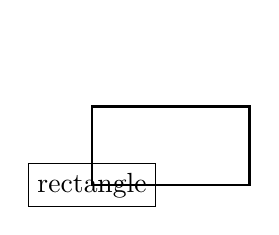
\begin{tikzpicture}
    \coordinate (O) (2,2);
    \node[draw, rectangle] (rec) at (0,0) {rectangle};	% here the coordinate (0,0) is the bottom left point's coor.
    \draw[thick] (O) rectangle ++(2,1);
\end{tikzpicture}
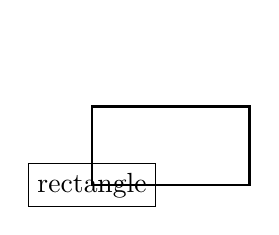
\begin{tikzpicture}
    \coordinate (O) (2,2);
    \node[draw, rectangle] (rec) at (0,0) {rectangle};	
    \draw[thick] (O) rectangle (2,1);
\end{tikzpicture}
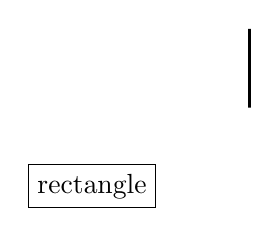
\begin{tikzpicture}
    \node[draw, rectangle] (rec) at (0,0) {rectangle};	
    \draw[thick] (2,2) rectangle (2,1);
\end{tikzpicture}
\begin{tikzpicture}
    \node[draw, rectangle] (rec) at (0,0) {rectangle};	
    \draw[thick] (2,2) rectangle ++(2,1);
\end{tikzpicture}
The \emph{rectangle} command requires the absolute corner coords. 
You are giving the increments in the second coordinates. So we can see
in the third above plot, it looks like a line, because the second coordinate
is not given as increments.

%%%%%%%%%%%%%%%%%%%%%%%%
\subsubsection{grid}
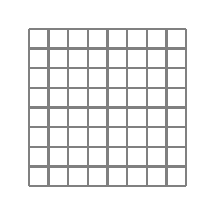
\begin{tikzpicture}
    \draw[step=0.25cm,gray,thick](-1,-1) grid(1,1);
\end{tikzpicture}

%%%%%%%%%%%%%%%%%%%%%%%%
\subsubsection{parabola, sin, cos}
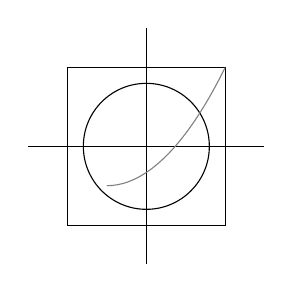
\begin{tikzpicture}
    \draw (-1.5, 0) -- (1.5, 0);
    \draw (0, -1.5) -- (0, 1.5);
    \draw (0, 0) circle (.8cm);
    \draw (-1, -1) rectangle (1, 1);
    \draw[gray] (-.5, -.5) parabola (1, 1);
\end{tikzpicture}
\tikz\draw[x=5pt, y=5pt] (0,0) parabola bend (4,16) (6,12);

{\bf sin} and {\bf cos} add a sine or cosine curve in the interval 
[0, $\pi/2$] such that the previous current point is at the start of the
curve and the curve ends at the given end point following it.

\tikz\draw[x=10pt,y=10pt] (0,0) sin (1,1) cos (2,0) sin (3,-1) cos (4,0)
			  (0,1) cos (1,0) sin (2,-1) cos (3,0) sin (4,1);
%%%%%%%%%%%%%%%%%%%%%%%%
\subsubsection{arc}
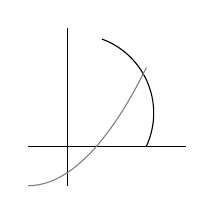
\begin{tikzpicture}
    \draw (-.5, 0) -- (1.5, 0);
    \draw (0, -.5) -- (0, 1.5);
    \draw (1, 0) arc (-25:70:1cm);
    \draw[gray] (-.5, -.5) parabola (1, 1);
\end{tikzpicture}
\hfill
\tikz\draw (0,0) arc (0:180:1cm);
\hfill
\hfill
\tikz\draw[fill=gray!50] (4, 0) -- +(30:1cm) arc (30:60:1cm) -- cycle;
\hfill
\tikz\draw[fill=gray!50] (4, 0) -- +(30:2cm) arc (30:60:1cm) -- cycle;

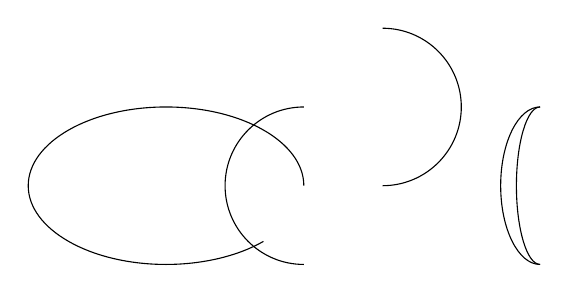
\begin{tikzpicture}
    \draw (0,1) arc (90:270:1);
    \draw (1,0) arc (-90:90:1);
    \draw (3,1) arc (90:270:0.3 and 1);
    \draw (3,1) arc (90:270:0.5 and 1);
    \draw (0,0) arc (0:315:1.75cm and 1cm);
\end{tikzpicture}


%%%%%%%%%%%%%%%%%%%%%%%%
\subsubsection{Arrow}
To draw the arrow head whthin the line, use \emph{decorate} option. \\
(need \verb|\usetikzlibrary{decorations.markings}|)


\begin{tikzpicture}
    \tikzstyle arrowstyle=[scale=1]
    \tikzstyle directed=[postaction={decorate,decoration={markings,
    mark=at position .65 with {\arrow[arrowstyle]{stealth}}}}]
    \tikzstyle reversed directed=[postaction={decorate, decoration={markings,
    mark=at position .65 with {\arrowreversed[arrowstyle]{stealth}}}}]

    \draw [red, ultra thick, directed] (0,0) -- (2,2);
\end{tikzpicture}

%%%%%%%%%%%%%%%%%%%%%%%%
\subsubsection{control points}
Control points in drawing.

\hfill
\begin{tikzpicture}
    \fill[GreenYellow!35] (-5pt, -5pt) rectangle (2cm+5pt, 2cm+5pt);

    \filldraw [gray] (0,0) circle (2pt)
		     (1,1) circle (2pt)
		     (2,1) circle (2pt)
		     (2,0) circle (2pt);
    \draw (0,0) .. controls (1,1) and (2,1) .. (2,0);

    \footnotesize
    \draw[shift={(2,1)}, xshift=0.5cm]
    node [right, text width=12cm, rounded corners, fill=blue!20,inner sep=1ex]
    {
	\begin{lstlisting}[language=TeX]
\begin{tikzpicture}
    \filldraw [gray] (0,0) circle (2pt)
		     (1,1) circle (2pt)
		     (2,1) circle (2pt)
		     (2,0) circle (2pt);
    \draw (0,0) .. controls (1,1) and (2,1) .. (2,0);
\end{tikzpicture}
	\end{lstlisting}
    };
\end{tikzpicture}

\hfill
\begin{tikzpicture}
    \fill[GreenYellow!35] (-1.5cm-5pt, -1.5cm-5pt) rectangle (1.5cm+5pt, 1.5cm+5pt);

    \draw (-1.5,0) -- (1.5,0);
    \draw (0,-1.5) -- (0,1.5);
    \draw (-1,0) .. controls (-1,0.555) and (-0.555,1) .. (0,1)
		 .. controls (0.555,1) and (1,0.555) .. (1,0);

    \footnotesize
    \draw[shift={(1.5,0)}, xshift=0.5cm]
    node [right, text width=12cm, rounded corners, fill=blue!20,inner sep=1ex]
    {
	\begin{lstlisting}[language=TeX]
\begin{tikzpicture}
    \draw (-1.5,0) -- (1.5,0);
    \draw (0,-1.5) -- (0,1.5);
    \draw (-1,0) .. controls (-1,0.555) and (-0.555,1) .. (0,1)
		 .. controls (0.555,1) and (1,0.555) .. (1,0);
\end{tikzpicture}
	\end{lstlisting}
    };
\end{tikzpicture}

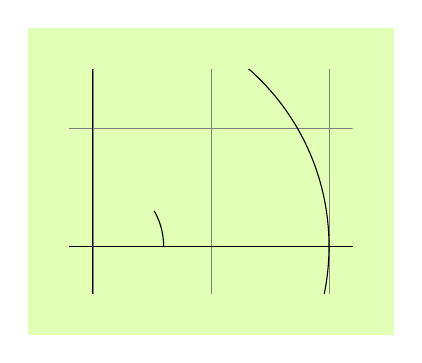
\begin{tikzpicture}[scale=3]
    \fill[GreenYellow!35] (-.1cm-5pt, -.2cm-5pt) rectangle (1.1cm+5pt, 0.75cm+5pt);

    \clip (-0.1,-0.2) rectangle (1.1,0.75);
    \draw[step=.5cm,gray,very thin] (-1.4,-1.4) grid (1.4,1.4);
    \draw (-1.5,0) -- (1.5,0);
    \draw (0,-1.5) -- (0,1.5);
    \draw (0,0) circle (1cm);
    \draw (3mm,0mm) arc (0:30:3mm);
\end{tikzpicture}

If you use relative control points, then the first one is relative to the
start node, while the second one is relative to the end node.

%%%%%%%%%%%%%%%%%%%%%%%%
\subsubsection{shade}
\verb|\shade| and \verb|\shadedraw|

\tikz \shade (0,0) rectangle (2,1)  (3,0.5) circle (0.5cm);

The default shading is a smooth transition from gray to white. To use 
other colors, specify them in options:

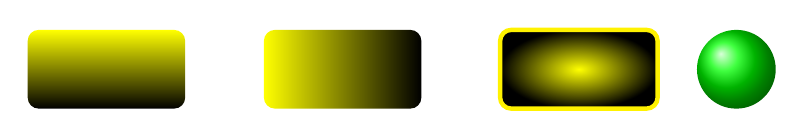
\begin{tikzpicture}[rounded corners, ultra thick]
    \shade [top color=yellow, bottom color=black] (0,0) rectangle +(2,1);
    \shade [left color=yellow, right color=black] (3,0) rectangle +(2,1);
    \shade [inner color=yellow, outer color=black, draw=yellow] (6,0) rectangle +(2,1);
    \shade [ball color=green] (9,.5) circle (0.5cm);
\end{tikzpicture}

%%%%%%%%%%%%%%%%%%%%%%%%
\subsubsection{+ sign}
\verb|+(1cm,0cm)| means ``1cm upwards from the previous specified position"; 
while \verb|++(0cm,2cm)| means ``2cm to the right of the previous specified
position, making this the {\bf new} specified position."

\tcbset{colback=brown!30}
\begin{tcolorbox}[width=4cm]
    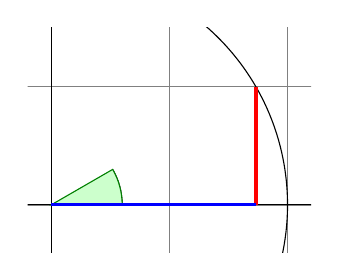
\begin{tikzpicture}[scale=3]
	\clip (-0.1,-0.2) rectangle (1.1,0.75);
	\draw[step=.5cm,gray,very thin] (-1.4,-1.4) grid (1.4,1.4);
	\draw (-1.5,0) -- (1.5,0);
	\draw (0,-1.5) -- (0,1.5);
	\draw (0,0) circle (1cm);
	\draw (3mm,0mm) arc (0:30:3mm);
	\filldraw[fill=green!20,draw=green!50!black] (0,0) -- (3mm,0mm) arc (0:30:3mm) -- cycle;
	\draw[red,very thick] (30:1cm) -- +(0,-0.5);
	\draw[blue,very thick] (30:1cm) ++(0,-0.5) -- (0,0);
\end{tikzpicture}
\end{tcolorbox}

Note the difference between \verb|+| and \verb|++| (see the code).

Using \verb|++|:

\begin{tikzpicture}
    \def\rectanglepath{-- ++(1,0) -- ++(0,1) -- ++(-1,0) -- cycle}
    \draw (0,0) \rectanglepath;
    \draw (1.5,0) \rectanglepath;
\end{tikzpicture}

Using \verb|+|:

\begin{tikzpicture}
    \def\rectanglepath{-- +(1,0) -- +(1,1) -- +(0,1) -- cycle}
    \draw (0,0) \rectanglepath;
    \draw (1.5,0) \rectanglepath;
\end{tikzpicture}

%%%%%%%%%%%%%%%%%%%%%%%%
\subsubsection{Intersection}
\verb/(<p> |- <q>)/ is ``the intersection of a vertical line through p and a horizontal line through q."

An intersection between a line going up from (1,0) and aline going from 
the origin throught (30:1cm).

\tcbset{colback=blue!20}
\begin{tcolorbox}
    \verb|\draw[very thick,orange] (1,0) -- (intersection of 1,0--1,1 and 0,0--30:1cm);|
\end{tcolorbox}

%%%%%%%%%%%%%%%%%%%%%%%%
\subsubsection{Miscellaneous}

\begin{tikzpicture}[line width=5pt]
    \draw (0,0) -- (1,0) -- (1,1) -- (0,0);
    \draw (2,0) -- (3,0) -- (3,1) -- cycle;
    \useasboundingbox (0,1.5);
\end{tikzpicture}
%%%%%%%%%%%%%%%%%%%%%%%%%%%%%%%%%%%%%%%%%%%%%%%%
\subsection{Coordinate Systems}
\begin{itemize}
    \item canvas
    \item xyz
    \item canvas polar
    \item xyz polar
    \item barycentric
	\[
	    {\alpha_1\vec{v}_1 + \alpha_2\vec{v}_2 + \cdots + \alpha_n\vec{v}_n} \over {\alpha_1 + \alpha_2 + \cdots + \alpha_n}
	    \]
    \item node
    \item intersection
    \item perpendicular
\end{itemize}
Any {\bf canvas} coordinate system requires explict dimensions (units)
while {\bf xyz} coordinate systems don't.

e.g.

\hfill
\begin{tikzpicture}
    \fill[GreenYellow!40] (-5pt,-5pt) rectangle (2cm + 5pt, 2cm + 5pt);

    \draw [help lines] (0,0) grid (2,2);

    \draw (0,0) -- (canvas polar cs:angle=30,radius=1cm);
    \draw (0,0) -- (xyz polar cs:angle=60, radius=1);

    \footnotesize
    \draw[shift={(2,1)},xshift=0.5cm]
    node [right, text width=12cm, rounded corners, fill=blue!20,inner sep=1ex]
    {
	\begin{lstlisting}[language=TeX]
\begin{tikzpicture}
  \draw [help lines] (0,0) grid (2,2);
  
  \draw (0,0) -- (canvas polar cs:angle=30,radius=1cm);
  \draw (0,0) -- (xyz polar cs:angle=60, radius=1);
\end{tikzpicture}
	\end{lstlisting}
    };
\end{tikzpicture}

\subsection{Options}
%%%%%%%%%%%%%%%%%%%%%%%%
\subsubsection{line width}
\tikz\draw[line width=2mm] (0,0)--(4,0);
\subsubsection{rotate}
\tikz\draw[rotate=45] (0,0) ellipse (16pt and 20pt);
\subsubsection{scale}
\tikz\draw[scale=1.5,rotate=75] (0,0) ellipse (10pt and 16pt);
\subsubsection{xscale, yscale}
\tikz\draw[xscale=1.5, yscale=0.5] (0,0) ellipse (10pt and 16pt);


%%%%%%%%%%%%%%%%%%%%%%%%%%%%%%%%%%%%%%%%%%%%%%%%
\subsection{node}
\tikz\draw(1,1) node{A} -- (2,2) node{B};
\hfill
\tikz\draw(1,1) node[circle, draw]{A} -- (2,2) node[circle,draw]{B};

%%%%%%%%%%%%%%%%%%%%%%%%
\subsubsection{label and pin}
\tikz[label distance=2mm]
\node[circle,fill=gray!45,label=above:12,label=right:3,label=below:6,label=left:9]{clock};
\hfill
\tikz[pin distance=4mm]\draw(1,1)
node[circle,fill=gray!45,pin=above:12,pin=right:3,pin=below:6,pin=left:9]{}
circle (1cm);

%%%%%%%%%%%%%%%%%%%%%%%%%%%%%%%%%%%%%%%%%%%%%%%%
\subsection{Styles}
tikzstyle:
\begin{itemize}
    \item every path
    \item every node
	\begin{itemize}
	    \item every \textless {\it shape} \textgreater node
	    \item every \textless {\it part name} \textgreater node part
	    \item every label
	    \item every pin
	    \item every pin edge
	\end{itemize}
    \item every to
    \item every curve
    \item every line
    \item every edge
    \item every snake
    \item every matrix
	\begin{itemize}
	    \item every cell
	\end{itemize}
    \item tree
	\begin{itemize}
	    \item every child
	    \item every child node
	    \item level \textless {\it number} \textgreater
	\end{itemize}
    \item every plot
\end{itemize}
When defining tikzstyle, there is no space allowed between the defined style and the definition.

\verb|\tikzstyle arrowstyle=[scale=1]|	\textbf{Corrected}. \\
\verb|\tikzstyle arrowstyle = [scale=1]|\textit{Wrong}.
%%%%%%%%%%%%%%%%%%%%%%%%%%%%%%%%%%%%%%%%%%%%%%%%
\subsection{plot}
%%%%%%%%%%%%%%%%%%%%%%%%
\subsubsection{gnuplot}
Tikz use \emph{gnuplot} to plot function, so to get right plot, we need to
install \emph{gnuplot} firstly. After first complining, we will get a
*.x.gnuplot file, run \emph{gnuplot} against this file, then compile tex
file again, we will get wanted plots.

difference between \verb|--plot| and \verb|plot|
\tikz\draw(0,1) -- (1,1) --plot coordinates {(2,0) (2, 1.5)};
\tikz\draw(0,1) -- (1,1) plot coordinates {(2,0) (2, 1.5)};

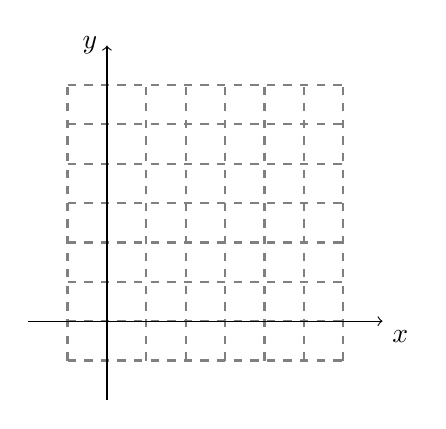
\begin{tikzpicture}[domain=0:2]
    \draw[thick,color=gray,step=0.5cm,dashed] (-0.5,-0.5) grid(3,3);
    \draw[->] (-1,0) -- (3.5,0) node[below right] {$x$};
    \draw[->] (0,-1) -- (0,3.5) node[left] {$y$};
    \draw plot[id=x] function{x*x};
\end{tikzpicture}

%%%%%%%%%%%%%%%%%%%%%%%%
\subsubsection{note on plots}
\begin{tikzpicture}
\node [anchor=west] (note) at (-1,3) {\Large Note};
\node [anchor=west] (water) at (-1,1) {\Large Water};
\begin{scope}[xshift=1.5cm]
    \node[anchor=south west,inner sep=0] (image) at (0,0)
    {\includegraphics[width=0.7\textwidth]{eiffel.jpg}};
    \begin{scope}[x={(image.south east)},y={(image.north west)}]
        \draw[red,ultra thick,rounded corners] (0.48,0.80) rectangle (0.55,0.95);
        \draw [-latex, ultra thick, red] (note) to[out=0, in=-120] (0.48,0.80);
        \draw [-stealth, line width=5pt, cyan] (water) -- ++(0.4,0.0);
    \end{scope}
\end{scope}
\end{tikzpicture}

%%%%%%%%%%%%%%%%%%%%%%%%%%%%%%%%%%%%%%%%%%%%%%%%%%%%%%%%%%%%%%%%%%%%%%%%
\section{Examples}
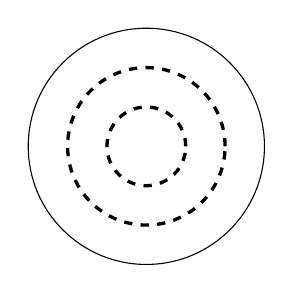
\begin{tikzpicture}
    \begin{scope}[very thick,dashed]
	\draw (0,0) circle (.5cm);
	\draw (0,0) circle (1cm);
    \end{scope}
    \draw[thin] (0,0) circle (1.5cm);
\end{tikzpicture}
\hfill

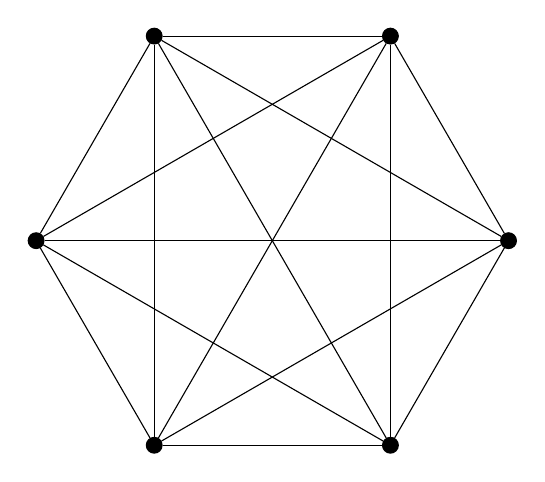
\begin{tikzpicture}[scale=1]
    \pgfmathsetmacro{\minsize}{0.2cm}
    \pgfmathsetmacro{\nodedist}{3}  
    \newcommand{\fillcolor}{black}

    \tikzstyle{every node}=[draw,shape=circle,minimum size=\minsize,inner sep=0]
    \foreach \x in {0,...,5}
	\node[fill=\fillcolor] (p\x) at (\x*60:\nodedist) {};	% (angle:radius)
    \foreach \x in {0,...,4}
    {
	\pgfmathtruncatemacro{\startvalue}{\x+1}
	\foreach \y in {\startvalue,...,5}
	    \draw (p\x) -- (p\y);
    }
\end{tikzpicture}
\hfill

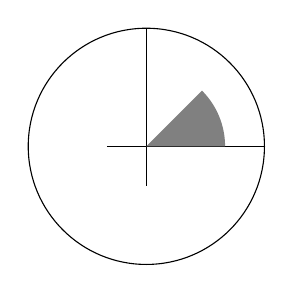
\begin{tikzpicture}
    \draw (-.5, 0)--(1.5,0);
    \draw (0, -.5)--(0, 1.5);
    \fill[gray] (0,0)--(1,0) arc (0:45:1cm) -- cycle;
    \draw[thin] (0,0) circle (1.5cm);
\end{tikzpicture}

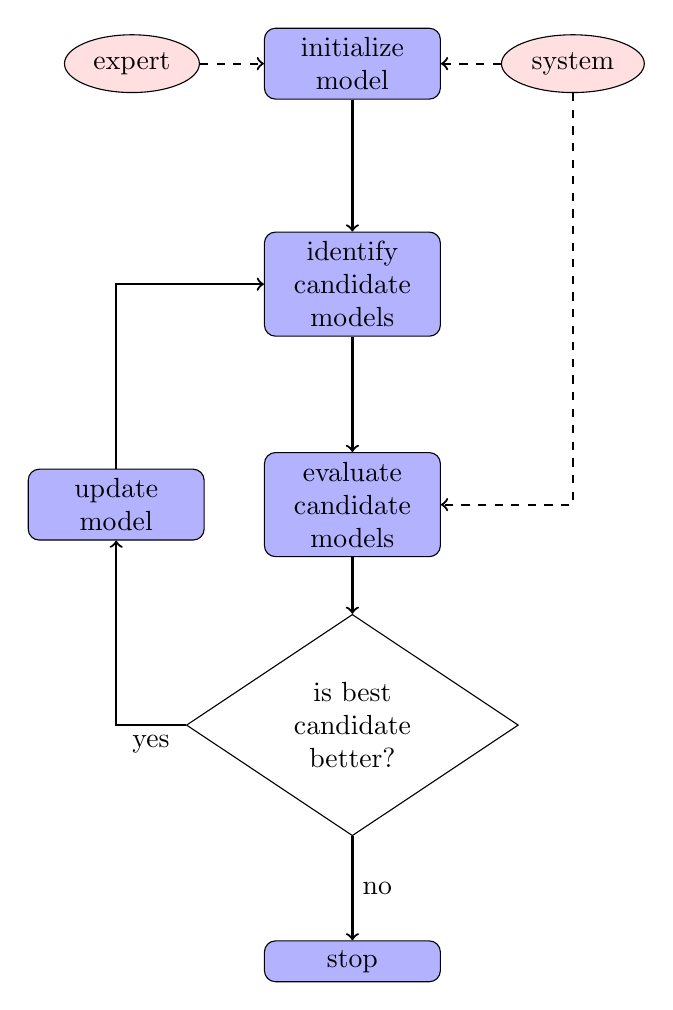
\begin{tikzpicture}[node distance=2.8cm, auto]
    \tikzstyle{block}=[rectangle, draw, rounded corners, text width=2cm,
    text centered, fill=blue!30];
    \tikzstyle{cloud}=[ellipse, draw, fill=pink!50, text centered];
    \tikzstyle{decision}=[diamond, draw,aspect=1.5,text width=2cm,text centered];
    \tikzstyle{line}=[->,black,thick,draw];
    % Place nodes
    \node [block] (init) {initialize model};
    \node [cloud, left of=init] (expert) {expert};
    \node [cloud, right of=init] (system) {system};
    \node [block, below of=init] (identify) {identify candidate models};
    \node [block, below of=identify] (evaluate) {evaluate candidate models};
    \node [block, left of=evaluate, node distance=3cm] (update) {update model};
    \node [decision, below of=evaluate] (decide) {is best candidate better?};
    \node [block, below of=decide, node distance=3cm] (stop) {stop};
    % Draw edges
    \path [line] (init) -- (identify);
    \path [line] (identify) -- (evaluate);
    \path [line] (evaluate) -- (decide);
    \path [line] (decide) -| node [near start] {yes} (update);
    \path [line] (update) |- (identify);
    \path [line] (decide) -- node {no}(stop);
    \path [line,dashed] (expert) -- (init);
    \path [line,dashed] (system) -- (init);
    \path [line,dashed] (system) |- (evaluate);
\end{tikzpicture}

\chapter{Customization}

%%%%%%%%%%%%%%%%%%%%%%%%%%%%%%%%%%%%%%%%%%%%%%%%%%%%%%%%%%%%%%%%%%%%%%%%
\section{Renewcommand}
You can modify default command by the command \verb|\renewcommand| to make
it fit your personal situation.
\begin{lstlisting}[language=TeX]
\renewcommand{\abstractname}{Executive Summary}	% Modify the title of your abstract
\renewcommand{\labelitemi}{$\triangleright$}
\renewcommand{\labelitemii}{\ding{43}}
\renewcommand{\labelitemiii}{\ding{44}}
\renewcommand{\labelitemiv}{\ding{45}}
\end{lstlisting}

%%%%%%%%%%%%%%%%%%%%%%%%%%%%%%%%%%%%%%%%%%%%%%%%
\subsection{Configuration}

%%%%%%%%%%%%%%%%%%%%%%%%
\subsubsection{Color}
\begin{lstlisting}[language=TeX]
\pagecolor[green!50!black!30]	% set page bg color
\end{lstlisting}
\subsubsection{Length}
\begin{lstlisting}[language=TeX]
\setlength{\paperwidth}{48in} 
\setlength{\paperheight}{36in}
\setlength{\sepwid}{0.024\paperwidth} % Separation width (white space) between columns
\setlength{\onecolwid}{0.22\paperwidth} % Width of one column
\setlength{\twocolwid}{0.464\paperwidth} % Width of two columns
\setlength{\threecolwid}{0.708\paperwidth} % Width of three columns
\setlength{\topmargin}{-0.5in} % Reduce the top margin size
\addtolength{\voffset}{-2.5cm}
\end{lstlisting}

%%%%%%%%%%%%%%%%%%%%%%%%%%%%%%%%%%%%%%%%%%%%%%%%%%%%%%%%%%%%%%%%%%%%%%%%
\section{New Command}
\begin{lstlisting}[language=TeX]
\newcommand{\SB}{Stony Brook}
\end{lstlisting}
Note that if type only \verb|\SB|, then the macro will eat up the following
space, producing ugly layout. To avoid that, you have to invoke it with an
empty statement after it: \verb|\SB{}|. 

The reason behind this is that \LaTeX ignores space directly after the
macro(which just stop the scanning for the macro's name). You need to break
that using either a protected space \verb|\SB\ | or an empty statement
\{\}.An empty statement is recommanded, as using a protected space can
generate nasty effects -- for example, if that protected space is directly
followed by a line break. In that case \LaTeX might pring two spaces
instead. Using an empty statement prevents this.

\verb|\def| command in {\bf plain \TeX{}} also do the work.
\begin{lstlisting}[language=TeX]
\def\intwrtx#1{\int_{-\infty}^{+\infty} #1 \,dx}
\end{lstlisting}
\def\intwrtx#1{\int_{-\infty}^{+\infty} #1 \,dx}
e.g.
$$ \intwrtx{f(x)}.$$

%%%%%%%%%%%%%%%%%%%%%%%%%%%%%%%%%%%%%%%%%%%%%%%%
\subsection{New Length}
\begin{lstlisting}[language=TeX]
\newlength{\onecolwid}{10cm}
\end{lstlisting}

or 

\begin{lstlisting}[language=TeX]
\newlength{\onecolwid}
\setlength{\onecolwid}{10cm}
\end{lstlisting}
%%%%%%%%%%%%%%%%%%%%%%%%%%%%%%%%%%%%%%%%%%%%%%%%
\subsection{New count}
\begin{lstlisting}[language=TeX]
\newcount{\opaqueness}
\end{lstlisting}

%%%%%%%%%%%%%%%%%%%%%%%%%%%%%%%%%%%%%%%%%%%%%%%%
\subsection{New dimension}
\begin{lstlisting}[language=TeX]
\newdimen{\offset}
\end{lstlisting}

%%%%%%%%%%%%%%%%%%%%%%%%%%%%%%%%%%%%%%%%%%%%%%%%%%%%%%%%%%%%%%%%%%%%%%%%
\section{Color}
\begin{lstlisting}[language=TeX]
\definecolor{mygreen}{rgb}{0,0.6,0}
\definecolor{mygray}{rgb}{0.5,0.5,0.5}
\definecolor{mypurple}{rgb}{0.58, 0, 0.82}
\end{lstlisting}

\subsection{xcolor}
\begin{lstlisting}[language=TeX]
\colorlet{LightRubinRed}{RubineRed!70!}	% xcolor; 70% or the intersity of 
% original RubineRed color. Or you can think of it as a mixture of 70% RubineRed
% and 30% white.
\colorlet{mycolor1}{green!10!orange!90!}
\definecolor{mycolor2}{HTML}{00F9DE}	% HTML model, the character A,B,C,D,E and F must be upper-case.
\end{lstlisting}

The color models that only \textbf{xcolor} support are:
\begin{itemize}
    \item \textbf{cmy} cyan, magenta, yellow
    \item \textbf{hsb} hue, saturation, brightness
    \item \textbf{HTML} RRGGBB
    \item \textbf{Gray} Grey scale, a number between 1 and 15.
    \item \textbf{wave} Wave length. Between 363 and 814    	
\end{itemize}

\chapter{Advanced}
\label{chap:Advanced}

%%%%%%%%%%%%%%%%%%%%%%%%%%%%%%%%%%%%%%%%%%%%%%%%%%%%%%%%%%%%%%%%%%%%%%%%
\section{Style}

%%%%%%%%%%%%%%%%%%%%%%%%%%%%%%%%%%%%%%%%%%%%%%%%
\subsection{Page Numbers}
How to change the numbering of pages:
\begin{lstlisting}{language=TeX}
\seccounter[page]{123}
\end{lstlisting}

How to remove all page numbers:
\begin{lstlisting}{language=TeX}
\pagestyle{empty}[page]{123}
\end{lstlisting}

\subsection{Citation}
How do I choose the square bracket or superscript style for citations:

%%%%%%%%%%%%%%%%%%%%%%%%%%%%%%%%%%%%%%%%%%%%%%%%
\subsection{Fonts}
\begin{lstlisting}[language=TeX]
\setmainfont{Times New Roman}	% serif fonts, for latin alphabetics
\setsansfont{helverica}	% latin non-serif alphabetics, usually for titles
\setmonofont{courier}	% same-width fonts, usually for code layout

% Chinese corresponding
\setCJKmainfont{simsun}
\setCJKsansfont{}
\setCJKmonofont{}   

% example: Linux Libertine
\setmainfont{LinLibertine\_R.otf}[
    BoldFont	= LinLibertine\_RZ.otf,
    ItalicFont	= LinLibertine\_RI.otf,
    BoldItalicFont = LinLibertine\_RZI.otf,
]
% sans-serif: Linux Biolinum
\setsansfont{LinLibertine\_R.otf}[
    BoldFont	= LinBiolimum\_RB.otf,
    ItalicFont	= LinBiolimum\_RI.otf,
    BoldItalicFont = LinBiolimum\_RBO.otf,
]
% typewriter type: Linux Libertine Mono
\setmonofont{LinLibertine\_M.otf}[
    BoldFont	= LinBiolimum\_MB.otf,
    ItalicFont	= LinBiolimum\_MI.otf,
    BoldItalicFont = LinBiolimum\_MBO.otf,
]

\setCJKmainfont[
    BoldFont	= Source Han Sans CN Medium,
    ItalicFont	= Adobe Kaiti Std R]
{Source Han Sans CN Light}
\setCJKsansfont[    % same as main
    BoldFont	= Source Han Sans CN Medium,
    ItalicFont	= Adobe Kaiti Std R]
{Source Han Sans CN Light}
\setCJKmonofont[
    BoldFont	= Source Han Sans CN Medium,
    ItalicFont	= Adobe Kaiti Std R]
{Source Han Sans CN Light}
\end{lstlisting}

%%%%%%%%%%%%%%%%%%%%%%%%%%%%%%%%%%%%%%%%%%%%%%%%%%%%%%%%%%%%%%%%%%%%%%%%
\section{Mode}
Using mode in \LaTeX{} allow one to choose different document class in one
tex file, for example:
\begin{lstlisting}[language=TeX]
\mode<presentation>{
    some preamble...
}

\mode<article>{
    preamble for article ...
}
\end{lstlisting}
Then if you compile a tex file (use the above one as input), then if the
documentclass is \textbf{beamer}, then mode \textbf{presentation} will be
used; if the documentclass is \textit{article}, then mode \textit{article}
will be choosed.

%%%%%%%%%%%%%%%%%%%%%%%%%%%%%%%%%%%%%%%%%%%%%%%%%%%%%%%%%%%%%%%%%%%%%%%%
\section{Adding note using tikz}
\newcommand{\annmark}[1]{%
    \textcolor{red}{$\langle$#1$\rangle$}%
}%

\newcommand{\ann}[1]{%
    \begin{tikzpicture}[remember picture, baseline=-0.75ex]%
        \node[coordinate] (inText) {};%
    \end{tikzpicture}%
    \marginpar{%
        \renewcommand{\baselinestretch}{1.0}%
        \begin{tikzpicture}[remember picture]%
            \definecolor{orange}{rgb}{1,0.5,0}%
            \draw node[fill=red!20,rounded corners,text width=\marginparwidth] (inNote){\footnotesize#1};%
    \end{tikzpicture}%
    }%
    \begin{tikzpicture}[remember picture, overlay]%
        \draw[draw = orange, thick]
            ([yshift=-0.2cm] inText)
                -| ([xshift=-0.2cm] inNote.west)
                -| (inNote.west);%
    \end{tikzpicture}%
}%

\setlength{\marginparwidth}{2.5cm}
\renewcommand{\baselinestretch}{1.3}

Freshness is the most important property for food \annmark{of course not 
for dry product }. And a good cooker will always keep food's freshness
and even enlarge the freshness using all kinds of methods.\ann{If one try to use spicy to hide all other flavor, then he must not a top cooker.} If you don't know how to cook a food, then the most obvious and simplest way is to boil it with water, which will sustain most of its freshness.

\chapter{Fantacy in \LaTeX{}}

\section{Display}
When you find something abnormal about mathmetics (wrong color), check that
if there is blank \$\$ pair without anything in it.

%%%%%%%%%%%%%%%%%%%%%%%%%%%%%%%%%%%%%%%%%%%%%%%%%%%%%%%%%%%%%%%%%%%%%%%%
\section{Package}
Updating package, if you update your texlive, and then encounter some errors
that you never met before, then it is the problem of old-packages. Remember 
to update corresponding packages so that everything work properly. Especially
when you install a new system and a new texlive but import old personal configuration.

%%%%%%%%%%%%%%%%%%%%%%%%%%%%%%%%%%%%%%%%%%%%%%%%
In \LaTeX, you can load a package many times, but the option list of each 
package loading must be a subset of the options given at the first loading (exception
\package{fontenc})

However sometimes packages might be loaded in the document class already, or
there are constraints in the package order that prevents the reordering of the 
packages. Then \command|\PassOptionsToPackage| helps. It can even
be loaded before \command|\documentclass|. It gives the specified 
options to the package without loading the package.

Adding the options to the global options can also be a solution, but it is not the
best strategy, because also other unrelated packages see that options. Unknown global 
options are ignored by package, but known are then executed with unintended side effects.

\subsection{physics \& imakeidx}
If I put package imakeidx before physics, then the compiler will complain
something like this:
\begin{verbatim}
(/usr/share/texlive/texmf-dist/tex/latex/imakeidx/imakeidx.sty
(/usr/share/texlive/texmf-dist/tex/latex/xkeyval/xkeyval.sty
(/usr/share/texlive/texmf-dist/tex/generic/xkeyval/xkeyval.tex
(/usr/share/texlive/texmf-dist/tex/generic/xkeyval/xkvutils.tex)))
(/usr/share/texlive/texmf-dist/tex/latex/tools/multicol.sty))
(/home/weibin/texmf/tex/latex/physics/physics.sty
(/home/weibin/texmf/tex/latex/l3packages/xparse/xparse.sty
(/home/weibin/texmf/tex/latex/l3kernel/expl3.sty
(/home/weibin/texmf/tex/latex/l3kernel/expl3-code.tex
! Missing number, treated as zero.
<to be read again> 
                   \pdftex_shellescape:D 
l.23338	    }
\end{verbatim}
But if I put physics before imakeidx, then no error happen.

%%%%%%%%%%%%%%%%%%%%%%%%%%%%%%%%%%%%%%%%%%%%%%%%
\subsection{tikz \& graphicx}
It looks like \textbf{tika} package will load \emph{graphicx} package
automatically, so if you load \emph{graphicx} package manually with some
options, it will cause problem. For example, if I load them as
\begin{verbatim}
\usepackage[dvips]{graphicx}
\usepackage{tikz}
\end{verbatim}
it will result in:
\begin{verbatim}
Non-PDF special ignored!
\end{verbatim}
On the other hand, if I load them as:
\begin{verbatim}
\usepackage{tikz}
\usepackage[dvips]{graphicx}
\end{verbatim}
We get such error:
\begin{verbatim}
! LaTeX Error: Option clash for package graphicx.
\end{verbatim}

So this should be the conflicts between different options used in loading
\emph{graphicx} package. If you load only the \textbf{tikz} package, 
then everything works perfectly.

% graphics
! Paragraph ended before \\Gin@iii was complete.    \\
You will encounter this error if you load \emph{graphics} rather than \emph{graphicx}.
%%%%%%%%%%%%%%%%%%%%%%%%%%%%%%%%%%%%%%%%%%%%%%%%
\subsection{xcolor}
\package{xcolor} option error:
\begin{verbatim}
! LaTeX Error: Option clash for package xcolor.
\end{verbatim}
Package \package{pgf} also load \package{xcolor}, so
\package{xcolor} should be loaded before \package{pgf} or 
other packages that loads \package{pgf}.

%%%%%%%%%%%%%%%%%%%%%%%%%%%%%%%%%%%%%%%%%%%%%%%%%%%%%%%%%%%%%%%%%%%%%%%%
\section{Environment}

%%%%%%%%%%%%%%%%%%%%%%%%%%%%%%%%%%%%%%%%%%%%%%%%
\subsection{gathered}
No blank line allowed with \emph{gathered} environment, otherwise, it will show
error message:
\begin{verbatim}
! Missing $ inserted.
<inserted text> $
\end{verbatim}

%%%%%%%%%%%%%%%%%%%%%%%%%%%%%%%%%%%%%%%%%%%%%%%%%%%%%%%%%%%%%%%%%%%%%%%%
\section{Options}
%%%%%%%%%%%%%%%%%%%%%%%%%%%%%%%%%%%%%%%%%%%%%%%%
\subsection{aligned}
In the \emph{aligned} environment, if you begin you equation with \textbf{square bracket},
they will not be output normally, because aligned env. is set by the \emph{amsmath} package to scan ahead for a positioning augument such as [t] of [p]. Material that's found there but doesn't meet this format is simply discarded.	

The possible solutions are:
\begin{itemize}
    \item Insert \verb|\relax| before the left square bracket. It will stop the bracket from being interpreted as an argument.
    \item Insert \{\} before the left square brackedt.
\end{itemize}

\chapter{Bibliography}
Things about citing bibliography.

% \input{}
% \include{hello_world/Package}
\end{document}
